\documentclass[9pt]{report}

\usepackage{talks}

\begin{document}


\sf%
\mbox{ }
\\[12pt]
\spc{{\LARGE\bfseries \color{MidnightBlue}{Pathfinder: }}}
\\[8pt]
\spc{\LARGE\bfseries \color{MidnightBlue}{Quasi-Newton variational inference}}
\\[36pt]
\noindent 
\spc{\large\bfseries \color{MidnightBlue}{Bob Carpenter}}
\\[2pt]
\spc{\small Center for Computational Mathematics}
\\[2pt]
\spc{\small Flatiron Institute}
\vfill 
\noindent 
\spc{\footnotesize October 2021}
\hfill 

\includegraphics[width=1.5in]{img/flatiron_logo.png}

\sld{Pathfinder}
\begin{itemize}
\item Lu Zhang, Bob Carpenter, Andrew Gelman, Aki
  Vehtari. 2021. Pathfinder: Parallel quasi-Newton variational
  inference. \textit{arXiv} 2108.03782.
  \begin{subitemize}
  \item under review at \textit{Journal of Machine Learning Research}
    \end{subitemize}
  \item it took about a year and a whole lot of meetings and revisions
    \begin{subitemize}
    \item Lu did all the heavy lifting and is on the job market in biostats
  \end{subitemize}
\item under development for Stan \hfill (me, Lu, Steve Bronder, Brian Ward)
\item ported (from R, pseudocode) to Julia and PyMC3 and Lu's talking to Pyro devs
\end{itemize}

\sld{Design for Stan integration}
\begin{center}
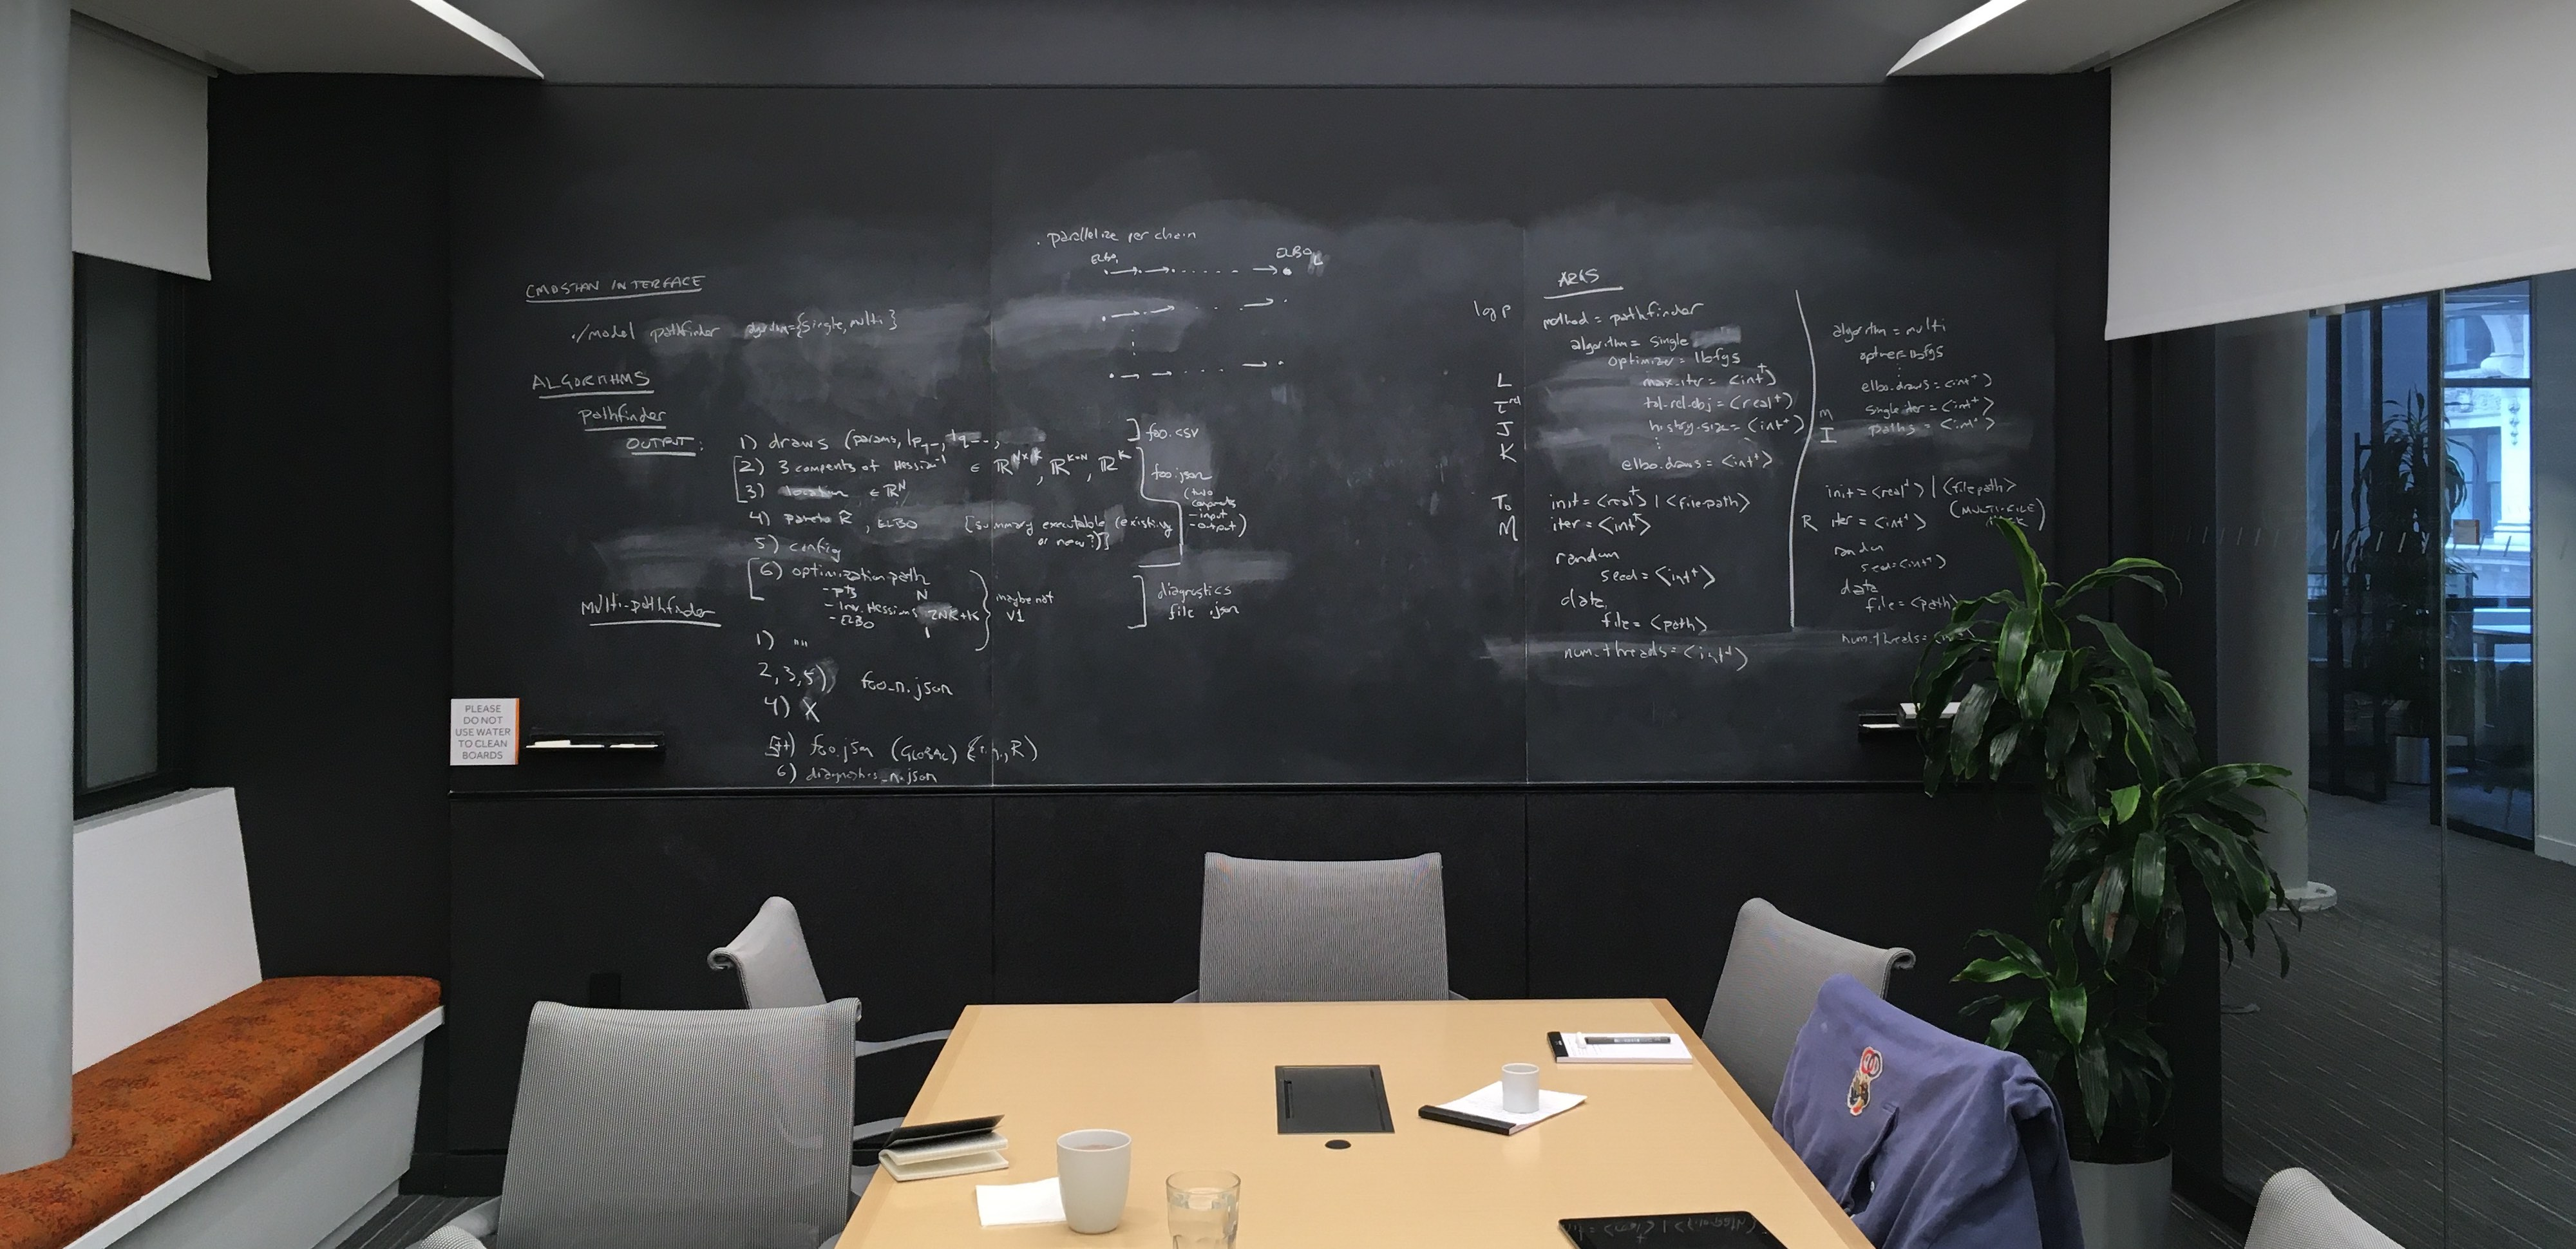
\includegraphics[width=0.9\textwidth]{img/stan-chalkboard.jpg}
\end{center}

\sld{Why am I so excited about Pathfinder?}
\begin{itemize}
\item vs.\ current state of the art in variational inference or Stan's ``burn-in''
  \begin{subitemize}
  \item 1--3 \myemph{orders of magnitude faster} without parallelization; 2--5 with
  \item less KL-divergence and closer Wasserstein-1 distance to target
    densities
  \item more robust to varying curvature and minor multimodality
  \end{subitemize}
\item rather than sampling the posterior via MCMC to calculate expectations
  \[
    \mathbb{E}[f(\theta) \mid y] \approx \frac{1}{M} \sum_{m=1}^M
    f(\theta^{(m)})
    \ \textrm{for} \ \theta^{(m)} \sim p(\theta \mid y),
  \]
  Pathfinder optimizes a normal variational approximation by
  \[
    \mu^*\!, \, \Sigma^*
    = \textrm{argmin}_{\mu, \Sigma} \
    \textrm{KL}\!\left[ \textrm{normal}(\theta \mid \mu, \Sigma)
      \ \big|\big| \
      p(\theta \mid y) \right]
    \]
\end{itemize}

\sld{Democratizing Bayesian inference}
\begin{itemize}
\item a primary goal is to \myemph{democratize Bayesian inference}
  \begin{subitemize}
  \item ``democratize'' is a term of art in software and to funders
  \item used in sense of being accessible to all (i.e., socializing)
  \end{subitemize}
\item another primary goal is to \myemph{push frontier} of fittable models
\item \myemph{black-box} methods
  \begin{subitemize}
  \item user codes a model in Stan language to define target log density
  \item algorithms agnostic to structure; in reality get under hood for hard cases
  \end{subitemize}
\item other goals
  \begin{subitemize}
  \item \myemph{expressiveness} of language, \
    \myemph{robustness} of inference, \
    \myemph{efficiency} and \myemph{scalability}, \
    easy \myemph{installation}, \
    thorough and useful \myemph{documentation}, \
    engaged \myemph{community}, \
    \myemph{maintainable} code base
    \end{subitemize}
\end{itemize}

\sld{Stan's black-box Bayesian inference}
\begin{itemize}
\item \myemph{full Bayesian inference} with Markov chain Monte Carlo (MCMC)
  \begin{subitemize}
  \item adaptive Hamiltonian Monte Carlo (gradient based)
  \item dense or diagonal metric (inverse mass matrix) estimation
  \end{subitemize}
\item \myemph{approximate Bayesian inference} with variational inference
  \begin{subitemize}
  \item autodiff variational inference (ADVI) 
  \item multivariate normal with dense or diagonal covar (mean field/full rank)
  \end{subitemize}
\item \myemph{Laplace approximation} with optimization
  \begin{subitemize}
  \item limited-memory BFGS (L-BFGS)
  \item does {\slshape not} adjust for Jacobian
  \end{subitemize}
\end{itemize}

\sld{Stan's models}
\begin{itemize}
\item Stan models define \myemph{log posterior densities} $\log p(\theta \mid y)$
  \begin{subitemize}
  \item require support $p(\theta \mid y) > 0$ for continuous parameters $\theta \in \mathbb{R}^N$
  \item observed data $y$ may be discrete or continuous
  \item constrained parameters are transformed (e.g., log transform scales $\sigma > 0$, Cholesky factor and log diagonal covariance matrices)
  \item change-of-variables adjustment implicitly applied under the hood
  \end{subitemize}
\item use \myemph{automatic differentiation} to compute $\nabla_{\!\theta} \, \log p(\theta \mid y)$
  \begin{subitemize}
  \item \myemph{dynamic} autodiff (like PyTorch, CppAD, Adol-C;  unlike TensorFlow)
  \item \myemph{much faster} than competition on CPU (TensorFlow, JAX, etc.)
  \item math and stats library much \myemph{richer} than TensorFlow Probability
  \end{subitemize}
\end{itemize}

\sld{Where do we draw samples?}
\begin{itemize}
\item from region where \myemph{density times volume} is highest
  \begin{subitemize}
  \item typically far from the max a posteriori (MAP) estimate
    \[
      \theta^* = \textrm{arg max}_{\theta} \, \log p(\theta \mid y)
    \]
  \end{subitemize}
\item consider drawing $y \in \mathbb{R}^N$ from a standard normal $y \sim \textrm{normal}(0, \textrm{I})$
  \begin{subitemize}
  \item i.e., dimensions i.i.d.\ std.\ normal, $y_n \sim \textrm{normal}(0, 1)$ for $n = 1, \ldots, N$
  \item maximum likelihood point is at mode $y = \begin{bmatrix} 0 & 0
      & \cdots & 0 \end{bmatrix}^{\top}$
  \end{subitemize}
\item squared Euclidean distance from origin (mode) is distributed
  \[
    \sum_{n = 1}^N y_n^2 \sim \textrm{ChiSq}(N)
  \]
\end{itemize}

\sld{Samples fall in $\textrm{ChiSq}(N)$ central interval}
\begin{center}
  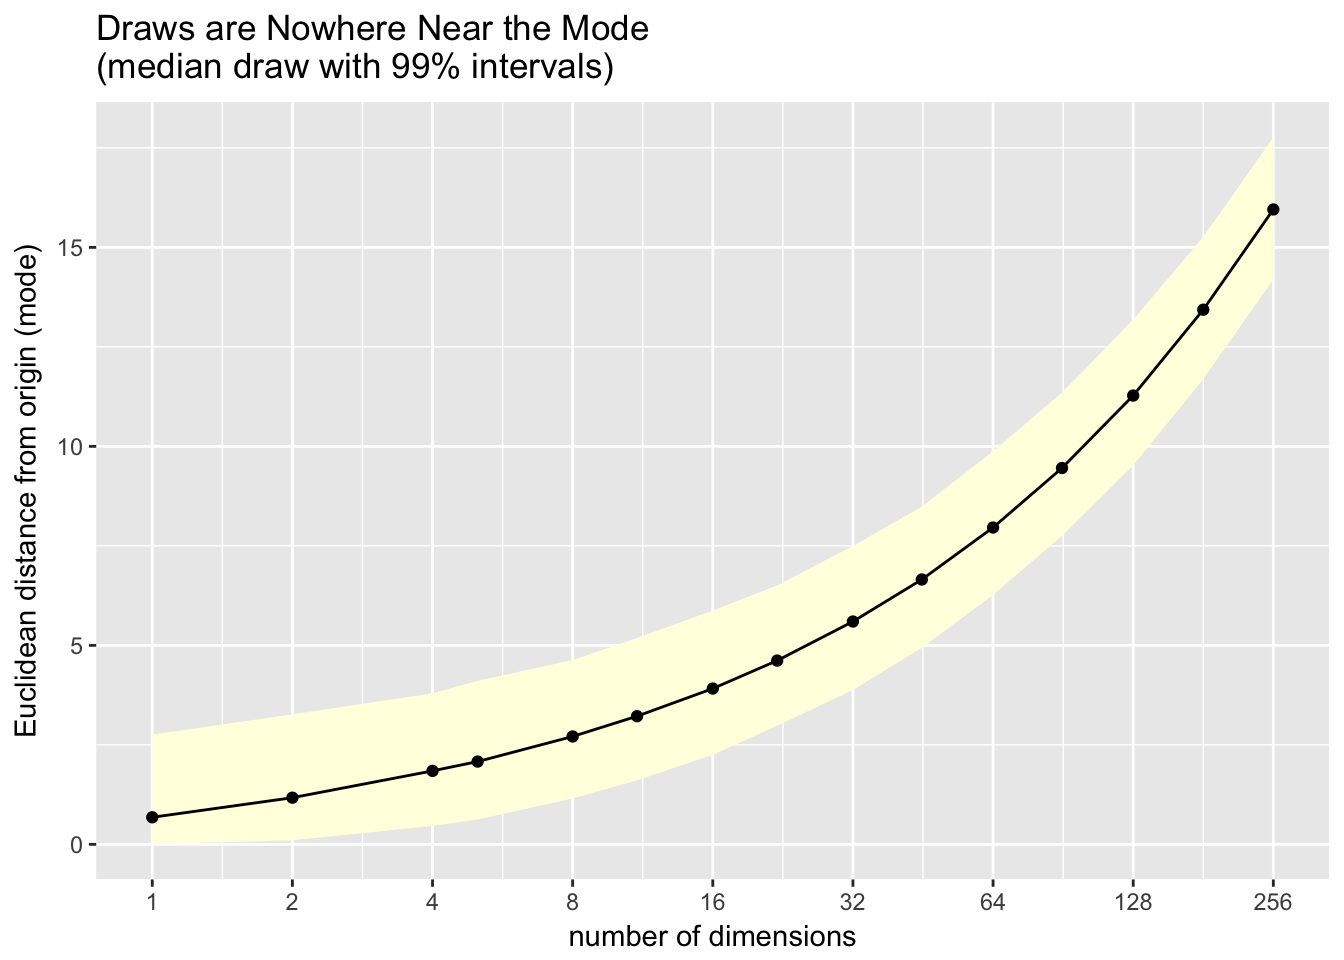
\includegraphics[width=0.6\textwidth]{img/normal-thin-shell.png}
\end{center}
\begin{subitemize}
  \item samples fall in a thin shell concentrated
    away from the origin (mode) as $N \rightarrow \infty$
  \end{subitemize}

\sld{Tail, body, and head of a distribution}
\vspace*{-12pt}
\begin{center}
\hspace*{2em}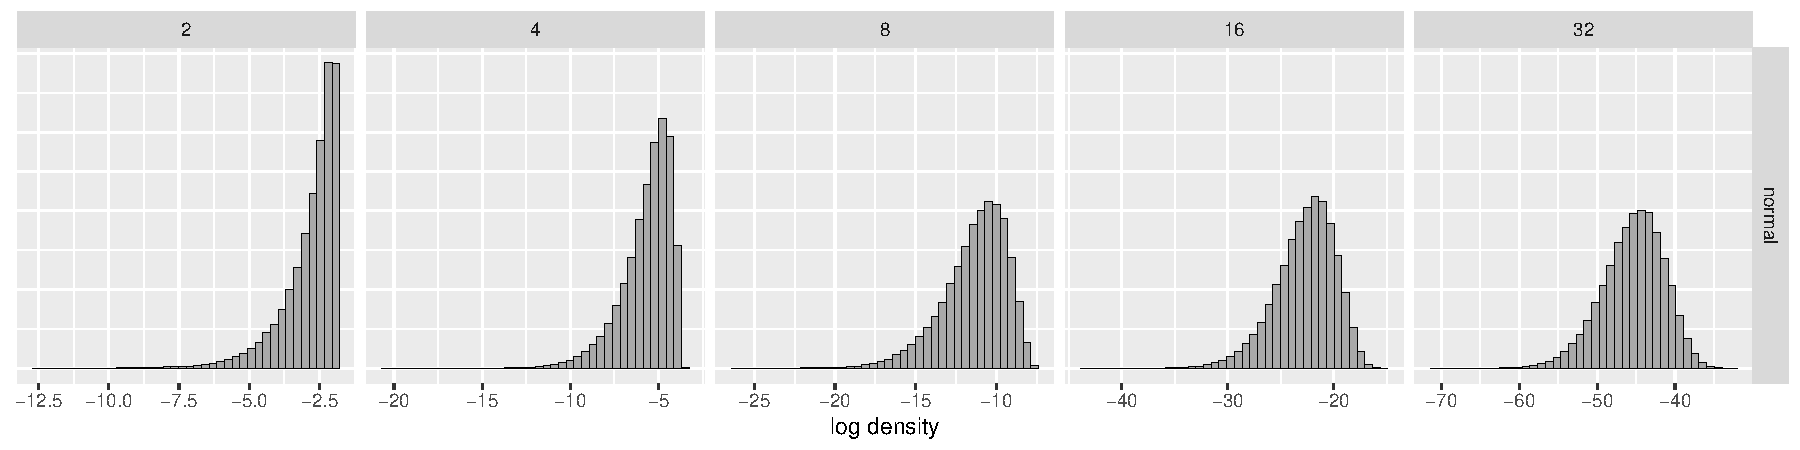
\includegraphics[width=\textwidth]{img/normal-posterior-log-density.pdf}
\end{center}
\vspace*{-12pt}
\begin{itemize}
\item
  \myemph{histograms of log densities} of draws from $N$-dimensional std.\ normal
\item sampling is \myemph{near expected log density} (equiv.\ neg.\ cond.\ entropy)
  \[
    \mathbb{E}\!\left[\log p(\Theta \mid y) \mid y\right]
    \ = \ 
    \int_{\Theta} p(\theta \mid y) \cdot \log p(\theta \mid y) \, \textrm{d}\theta
    \ = \
    -\textrm{H}[\Theta \mid y]
  \]
\item sampling is from \myemph{body}, lower density in \myemph{tail},
  higher in \myemph{head}
\end{itemize}

\sld{Typical draw has log density near expectation}
\begin{center}
  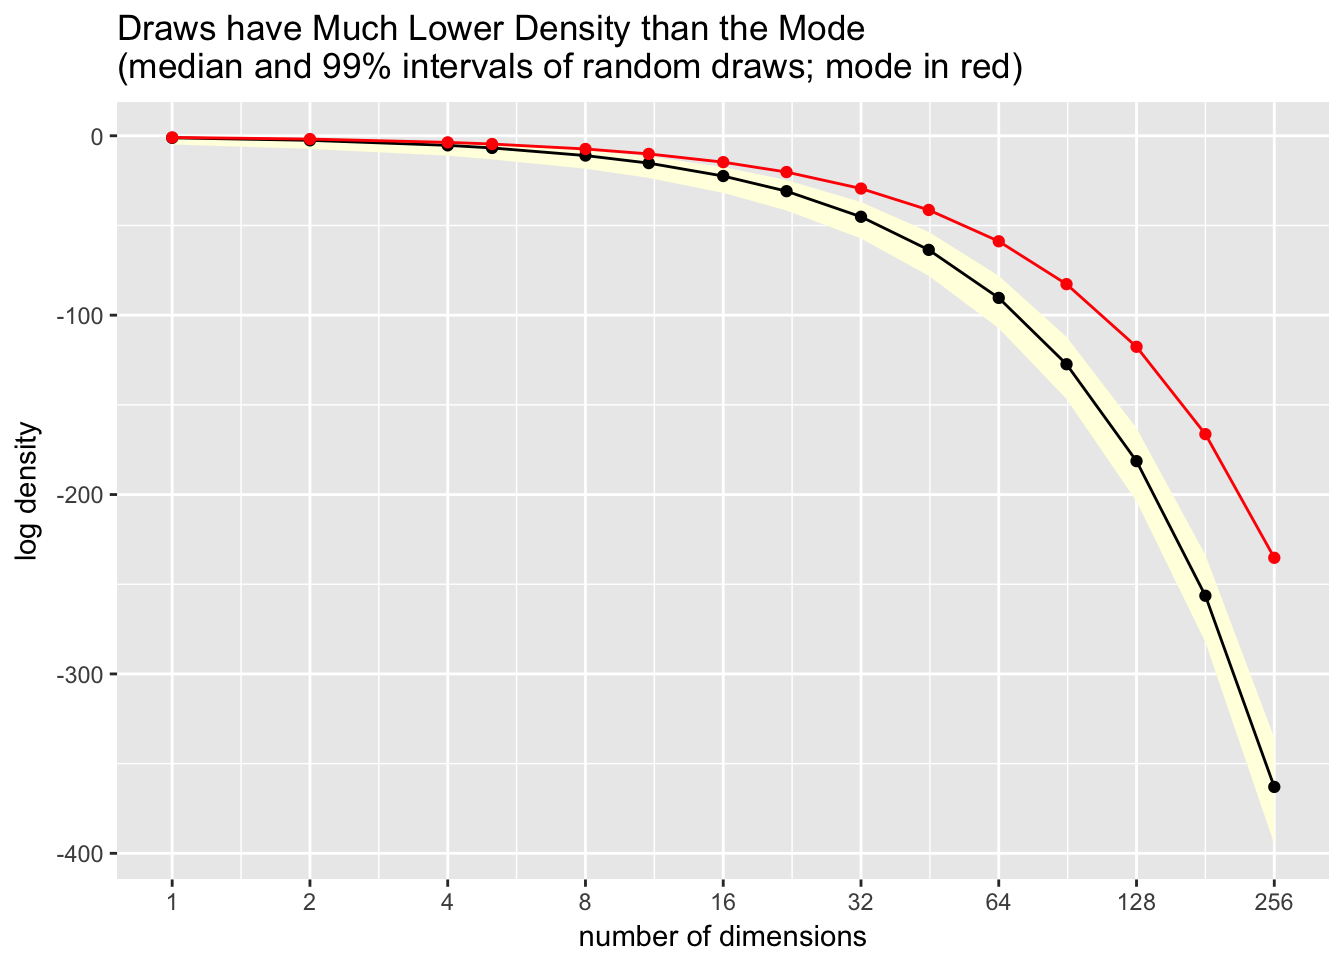
\includegraphics[width=0.5\textwidth]{img/99pct-mode-std-normal.png}
\end{center}
\begin{itemize}
\item yellow band is \myemph{99\% central interval}
  of log density for standard normal
\item red line is \myemph{log density of mode} (nearby is high
  density, low volume)
\end{itemize}


\sld{Motivation for Pathfinder: MCMC initialization}
\vspace*{-2pt}
\begin{center}
  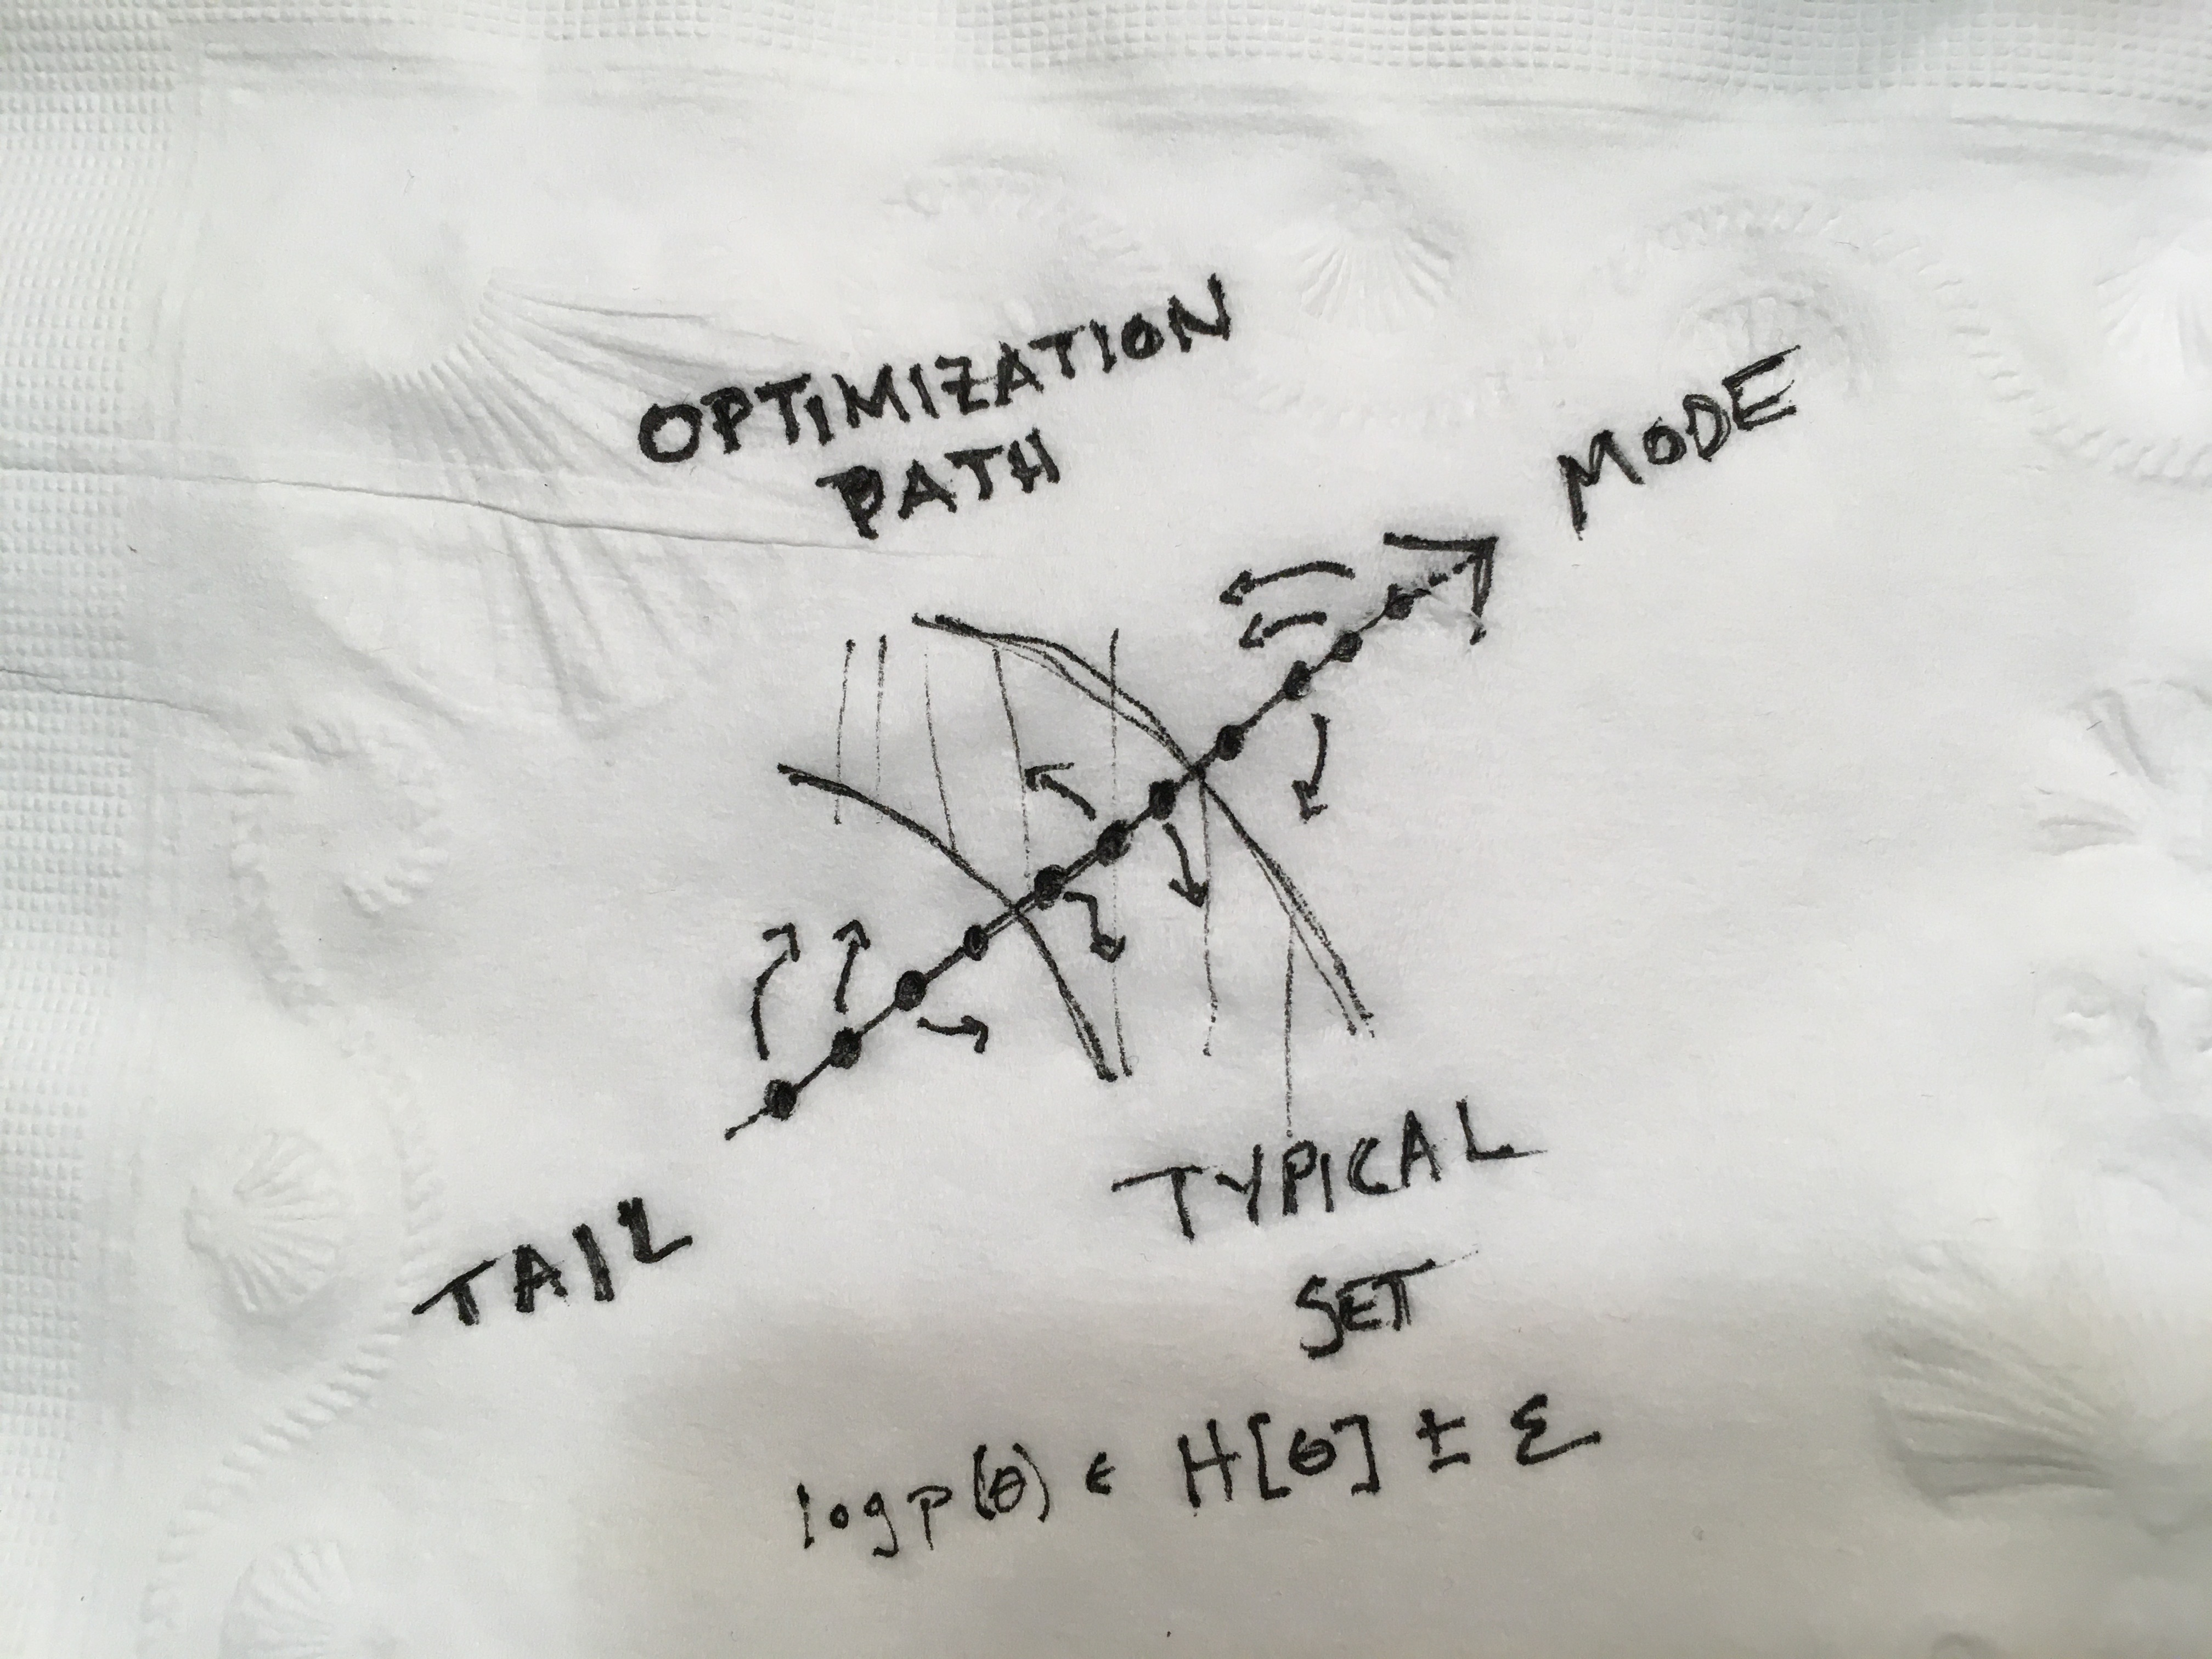
\includegraphics[width=0.35\textwidth]{img/napkin-adapt.jpg}
\end{center}
\vspace*{-4pt}
\begin{subitemize}
\item approximate random init.\ in the body makes Markov chain \myemph{approx.\ stationary}
\item \myemph{intermediate value} theorem: \myemph{optimization path} from tail \myemph{through body} to head
\item related to notion of \myemph{typical set} in information theory
  \begin{subitemize}
  \item points whose log density is within $\pm \epsilon$ of expected value
  \end{subitemize}
\end{subitemize}

\sld{Our first approach crashed}
\begin{center}
  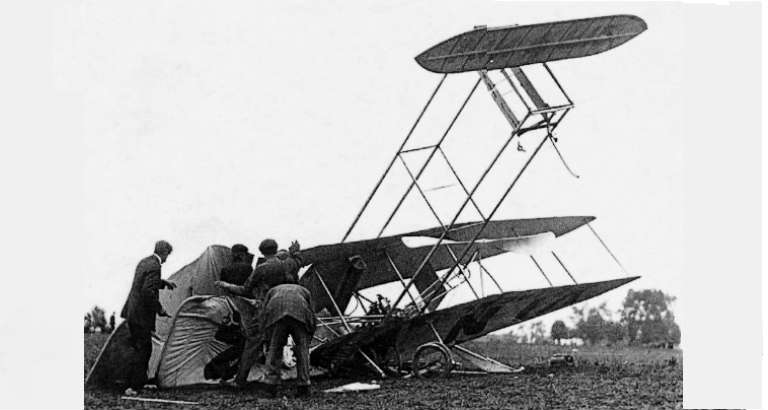
\includegraphics[width=0.9\textwidth]{img/wright-crash.jpg}
\end{center}

\sld{So did the second}
\begin{center}
  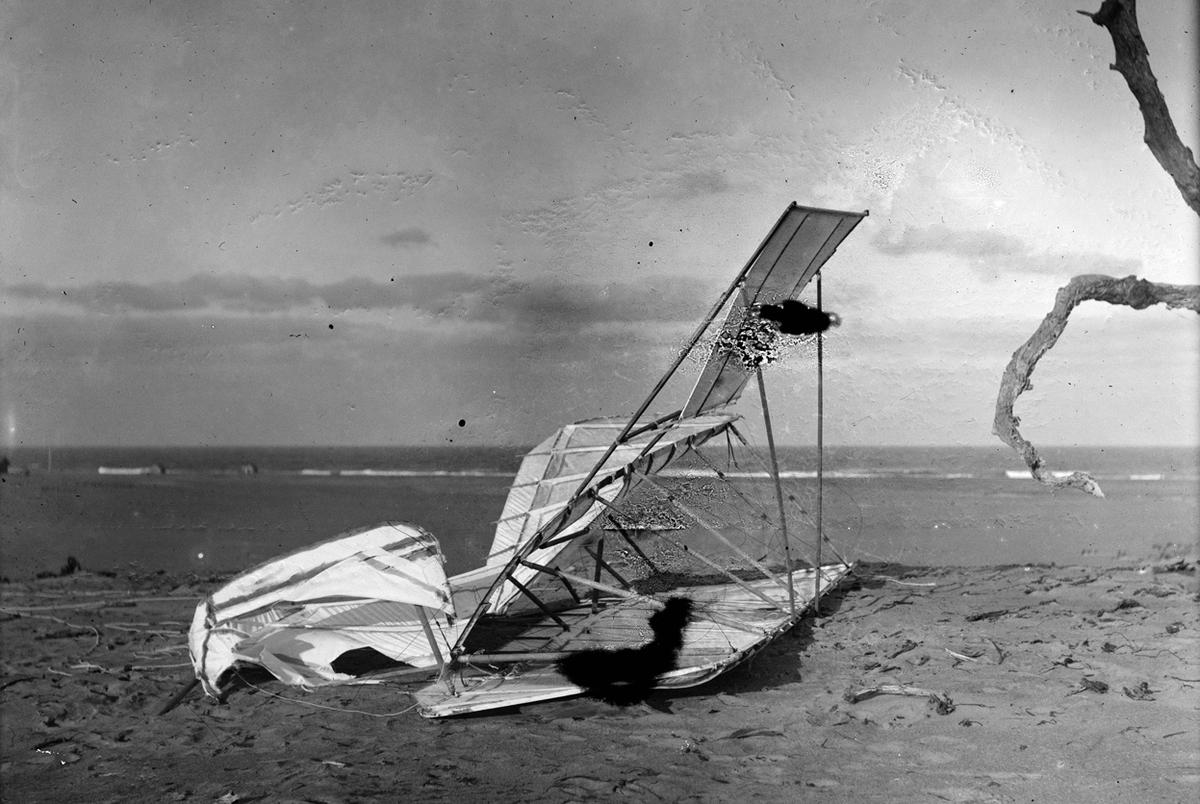
\includegraphics[width=0.7\textwidth]{img/wright-crash-2.jpg}
\end{center}

\sld{Failed attempts}
\begin{itemize}
\item run \myemph{optimization} to generate a trajectory of points
\item for each point, evaluate if its log density is near expectation 
\end{itemize}
\begin{enumerate}
\item run an MCMC chain for each point
  \begin{subitemize}
  \item from \myemph{tail}, draws trend up; from \myemph{head} trend down; in \myemph{body} bounce 
  \item but MCMC is slow, hard to adapt, and \myemph{intrinsically sequential}
  \end{subitemize}
\item estimate surface area of level set around a point to estimate volume
  \begin{subitemize}
  \item choose points whose \myemph{density times approximate volume} is high
  \item better, but still \myemph{not robust} to our \myemph{50+ test models}
  \end{subitemize}
\end{enumerate}

\sld{Third time's the charm}
\begin{center}
  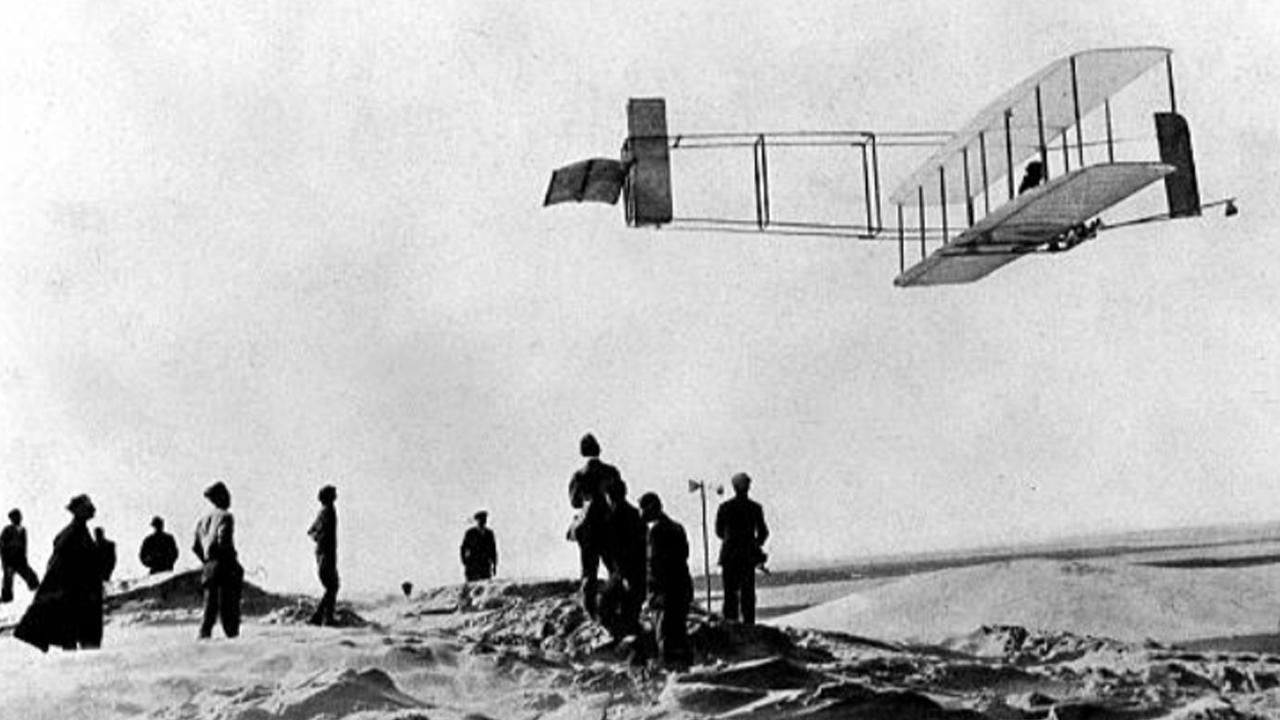
\includegraphics[width=0.8\textwidth]{img/wright-success.jpg}
\end{center}

\sld{Pathfinder basics}
\begin{itemize}
\item for each point on the optimization trajectory
\end{itemize}
\begin{enumerate}
\item[3.] evaluate the KL-divergence of an approximate normal
  \begin{subitemize}
  \item center a \myemph{multivariate normal approximation} (quadratic) on the point on the trajectory
  \item set covariance to \myemph{approximate inverse Hessian} from
    L-BFGS
    \begin{subitemize}
    \item low-rank outer product plus diagonal
    \end{subitemize}
  \item evaluate \myemph{KL-divergence from approximation to target density}
    \begin{subitemize}
    \item use \myemph{Monte Carlo} draws from approximation plus analytic normal entropy
    \end{subitemize}
  \item draw from approximation with lowest KL-divergence
  \end{subitemize}
\end{enumerate}

\sld{Logistic regression posterior example}
\vspace*{-6pt}
\begin{center}
  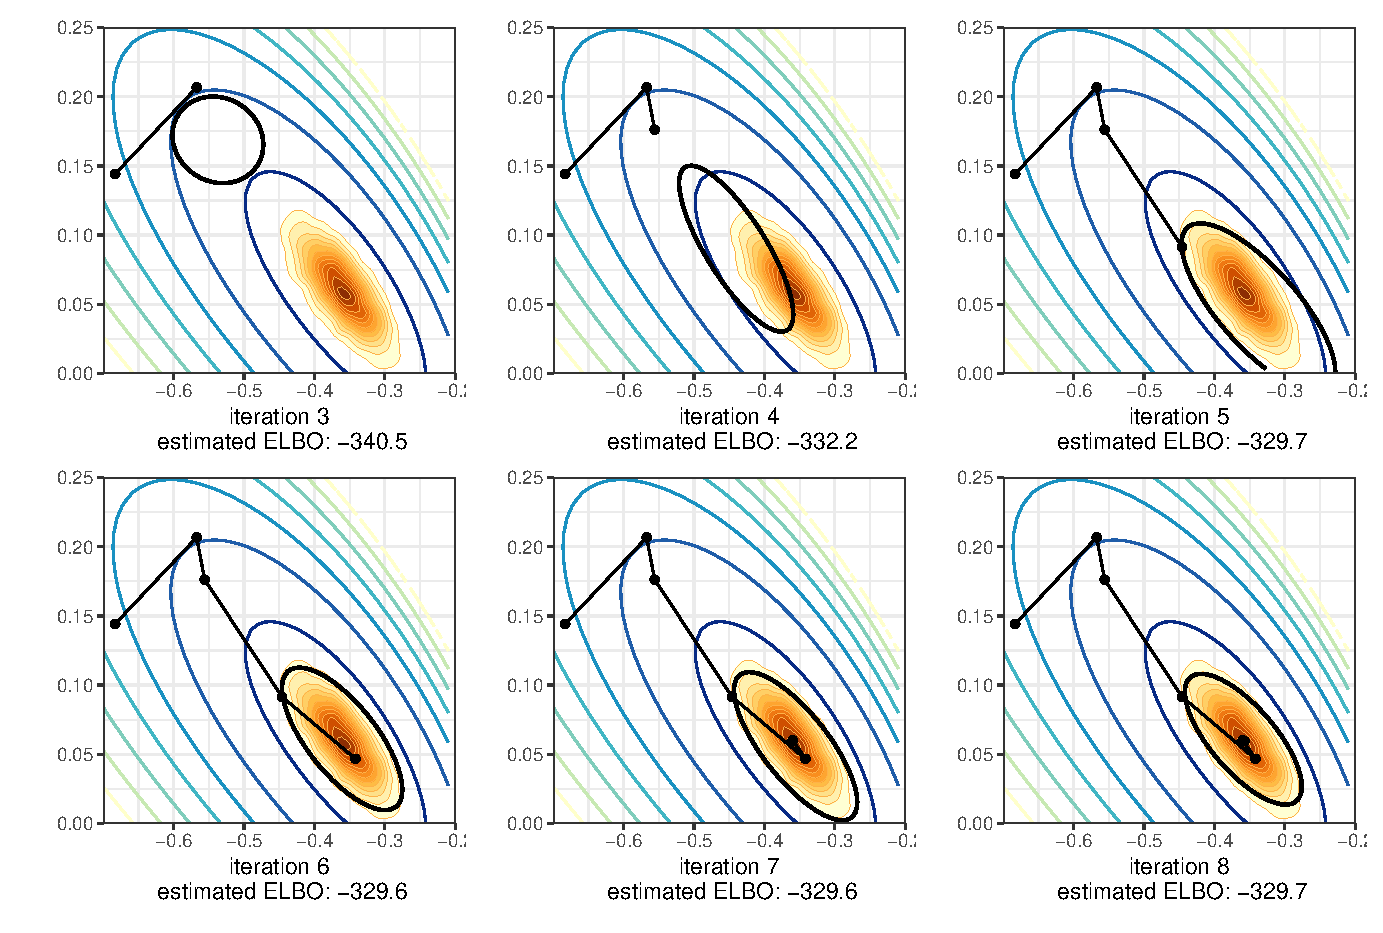
\includegraphics[width=0.6\textwidth]{img/logit_example.eps}
\end{center}
\vspace*{-6pt}
\begin{subitemize}
\item orange is target density, black ellipses the approximation
  \vspace*{-4pt}
\item ELBO is equal to negative KL divergence plus constant; optimized at mode giving Laplace approx.
\end{subitemize}

\sld{Neal's funnel posterior example}
\vspace*{-6pt}
\begin{center}
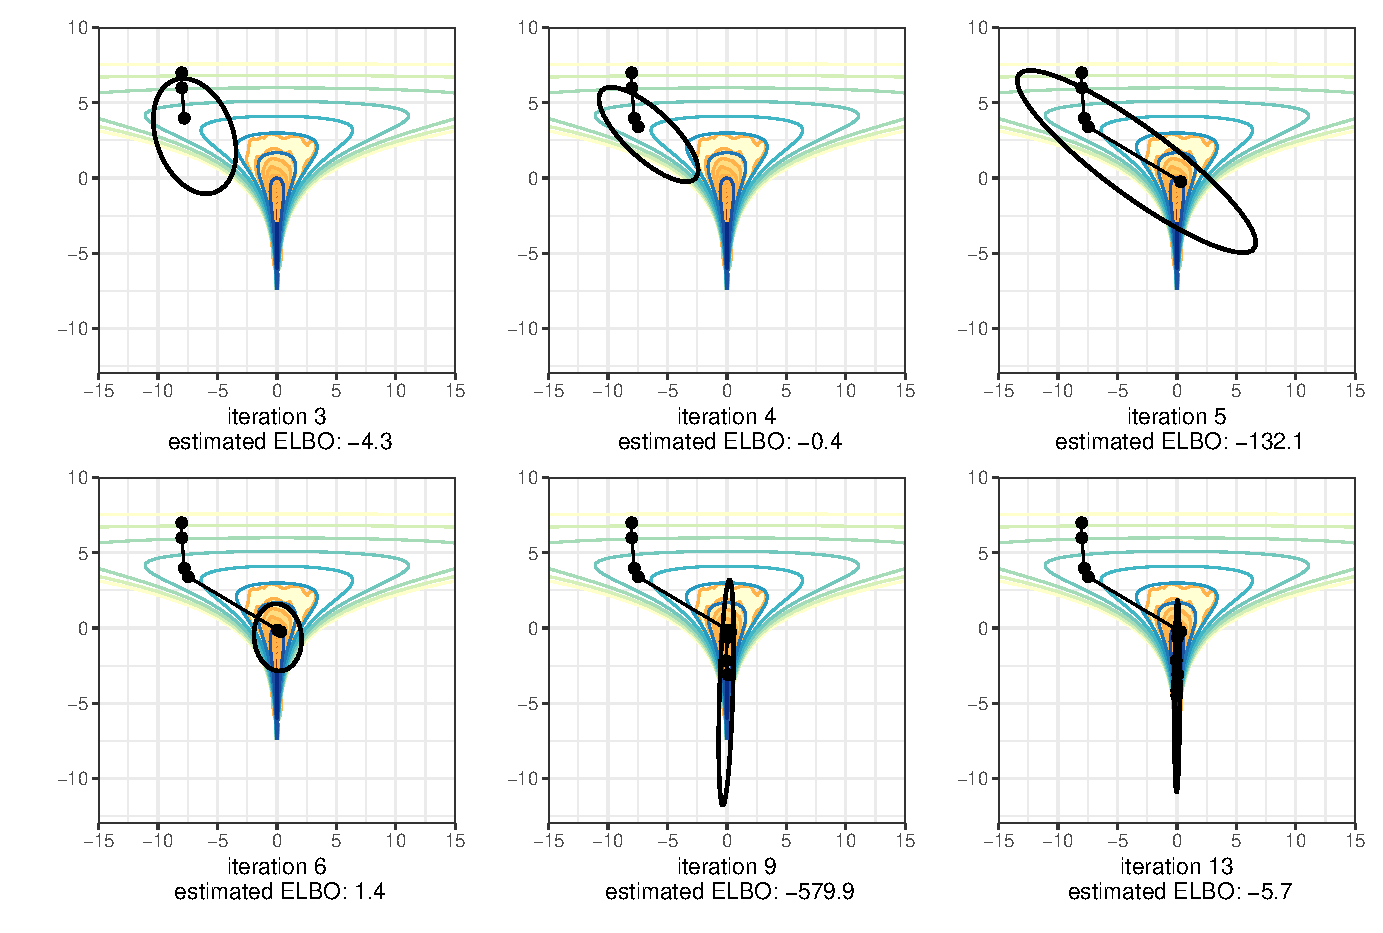
\includegraphics[width=0.6\textwidth]{img/funnel_example.eps}
\end{center}
\vspace*{-6pt}
\begin{subitemize}
\item no mode, just a pole as $y \rightarrow -\infty$ and $x \rightarrow 0$
\item Pathfinder selects approximation (lower left) within body
\end{subitemize}


\sld{Oops, we built a variational method}
\begin{itemize}
\item given a \myemph{target posterior} $p(\theta \mid y)$
\item \myemph{variational inference} assumes an \myemph{approximating} density
  \\ $q(\theta \mid \phi)$ with parameters $\phi$
\item variational approximation minimizes KL-divergence to target density
  \[
    \phi^*
    = \textrm{argmin}_{\phi} \
    \textrm{KL}\!\left[q(\theta \mid \phi) \,\bigg|\bigg|\, p(\theta \mid y)\right]
  \]
\end{itemize}

\sld{L-BFGS-derived normal approximation}
\begin{itemize}
\item Pathfinder uses a \myemph{multivariate normal} approximation on \myemph{unconstrained parameters}
  \[
    q(\theta \mid \phi) = \textrm{multi-normal}(\theta \mid \mu, \Sigma)
  \]
  \item \myemph{covariance} from L-BFGS's \myemph{low-rank plus diagonal} inverse
  Hessian approximation
  \[
    \Sigma = \textrm{diag}(\alpha) + \beta^{\top} \cdot \gamma \cdot
    \beta
  \]
  where
  \[
    \alpha \in \mathbb{R}^N, \quad
    \beta \in \mathbb{R}^{N \times J}, \quad
    \gamma \in \mathbb{R}^{J \times J}
    \]
  for rank-$J$ L-BFGS
\end{itemize}

\sld{Evaluating KL-divergence with Monte Carlo}
\vspace*{-4pt}
  \begin{eqnarray*}
\null \qquad \textrm{KL}\!\left[q(\theta \mid \phi) \,\bigg|\bigg|\, p(\theta \mid y)\right]
  & = &
  \mathbb{E}_{q(\theta \mid \phi)}
        \!\left[ \log \frac{q(\theta \mid \phi)}{p(\theta \mid y)} \right]
  \\[6pt]
  & = &   \mathbb{E}_{q(\theta \mid \phi)}[\log q(\theta \mid \phi)]
        - \mathbb{E}_{q(\theta \mid \phi)}[\log p(\theta \mid y)]
 \\[6pt]
 & = &   - \textrm{H}\!\left[q(\theta \mid y)\right] - \mathbb{E}_{q(\theta \mid \phi)}[\log p(\theta, y)] + \textrm{const.}
  \\[6pt]
%  & = & - \textrm{H}\!\left[q(\theta \mid y)\right] - \int_{\theta} q(\theta \mid \phi) \cdot \log p(\theta, y) \, \textrm{d}\theta + \textrm{const.}
%  \\[4pt]
  & \approx & -\textrm{H}\!\left[q(\theta \mid \phi)\right] - \frac{1}{M} \sum_{m=1}^M \log p(\theta^{(m)}, y) + \textrm{const.}
  \end{eqnarray*}
  \vspace*{-6pt}
\begin{subitemize}
\item where $\theta^{(m)} \sim q(\theta \mid \phi)$ are \myemph{Monte Carlo
  draws} from (normal) approximation
  \item \myemph{minimizing KL} balances high entropy and containment within target
\item \myemph{analytic entropy} $\textrm{H}\!\left[q(\theta \mid y)\right]$ for normal family $q(\theta \mid \phi) = \textrm{normal}(\theta \mid \mu, \Sigma)$
\end{subitemize}

\sld{Quasi-Newton inverse Hessian optimization}
\begin{itemize}
\item L-BFGS approximates $N \times N$ inverse Hessians with diagonal plus rank $J$ outer product,
  \[
    \Sigma = \textrm{diag}(\alpha) + \beta^{\top} \cdot \gamma \cdot \beta
  \]
\item reduces matrix op time/space complexity from $\mathcal{O}(N^3)$ to $\mathcal{O}(N \cdot J^2)$
  \begin{subitemize}
  \item random draws for evaluating KL-divergence: $\theta \sim \textrm{normal}(\mu, \Sigma)$
  \item evaluating approximate log density: $f(\theta) = \log \textrm{normal}(\theta \mid \mu, \Sigma)$
  \item preconditioner in quasi-Newton optimization within L-BFGS
    \[
      \delta = \left( -\nabla^2 \log p(\theta \mid y)\right)^{-1} \cdot \nabla \log p(\theta \mid y)
    \]
    uses approximation for inverse Hessian, $\left( \nabla^2 \log p(\theta \mid y) \right)^{-1}$
    \end{subitemize}
\end{itemize}

\sld{Competitor I: Autodiff variational inference (ADVI)}
\begin{itemize}
\item state-of-art \myemph{black-box variational inference in Stan} (Kucukelbir++, \textit{JMLR})
\item $q(\theta \mid \phi) = \textrm{normal}(\theta \mid \mu, \Sigma)$ with $\Sigma$ \myemph{diagonal} (``mean field'') or \myemph{dense}
\item \myemph{stochastic gradient} descent on the ELBO objective, i.e., gradients
  \[
    \nabla_{\phi} \left( -\textrm{H}\!\left[q(\theta \mid \phi)\right] - \frac{1}{M} \sum_{m=1}^M \log p(\theta^{(m)}, y) \right)
  \]
  where $\theta^{(m)} \sim \textrm{normal}(\theta \mid \mu, \Sigma)$ drawn from approximating distribution
\item using \myemph{``reparameterization trick''} for gradients
\item poor \myemph{stability, convergence} with stochastic gradients
\item optimization through KL-divergence is \myemph{intrinsically serial}
\end{itemize}

\sld{Competitor II: Stan phase I warmup}
\begin{itemize}
\item Stan currently uses \myemph{75 HMC iterations} of its sampler for \myemph{phase I warmup} (aka ``burn-in'')
  \begin{subitemize}
  \item \myemph{no U-turn sampler} (NUTS) (adaptive number of leapfrog steps, multinomial sampling over path) 
  \item \myemph{unit metric} (inverse mass matrix)
  \item lightly \myemph{adapted step size}
  \item \myemph{max 1024} leapfrog steps per iteration
  \end{subitemize}
\item this is \myemph{sufficient} for most of our test problems 
\item but it can be \myemph{very expensive} in number of log density/gradient evals
\end{itemize}

\sld{posteriordb evaluation set}
\begin{itemize}
\item \myemph{posteriordb} has about 50 models \hfill (Magnusson et al.)
  \begin{subitemize}
  \item generalized linear models
  \item hierarchical GLMs
  \item differential equation inverse problems
  \item time-series and stochastic volatility models
  \item mixture models and hidden Markov models
  \item Gaussian processes
  \end{subitemize}
\item 10K \myemph{reference posterior draws} per model (thinned HMC chains)
\item \myemph{not carefully parameterized} for HMC (e.g., centered params.)
\end{itemize}

\sld{How much faster is Pathfinder?}
\begin{center}
  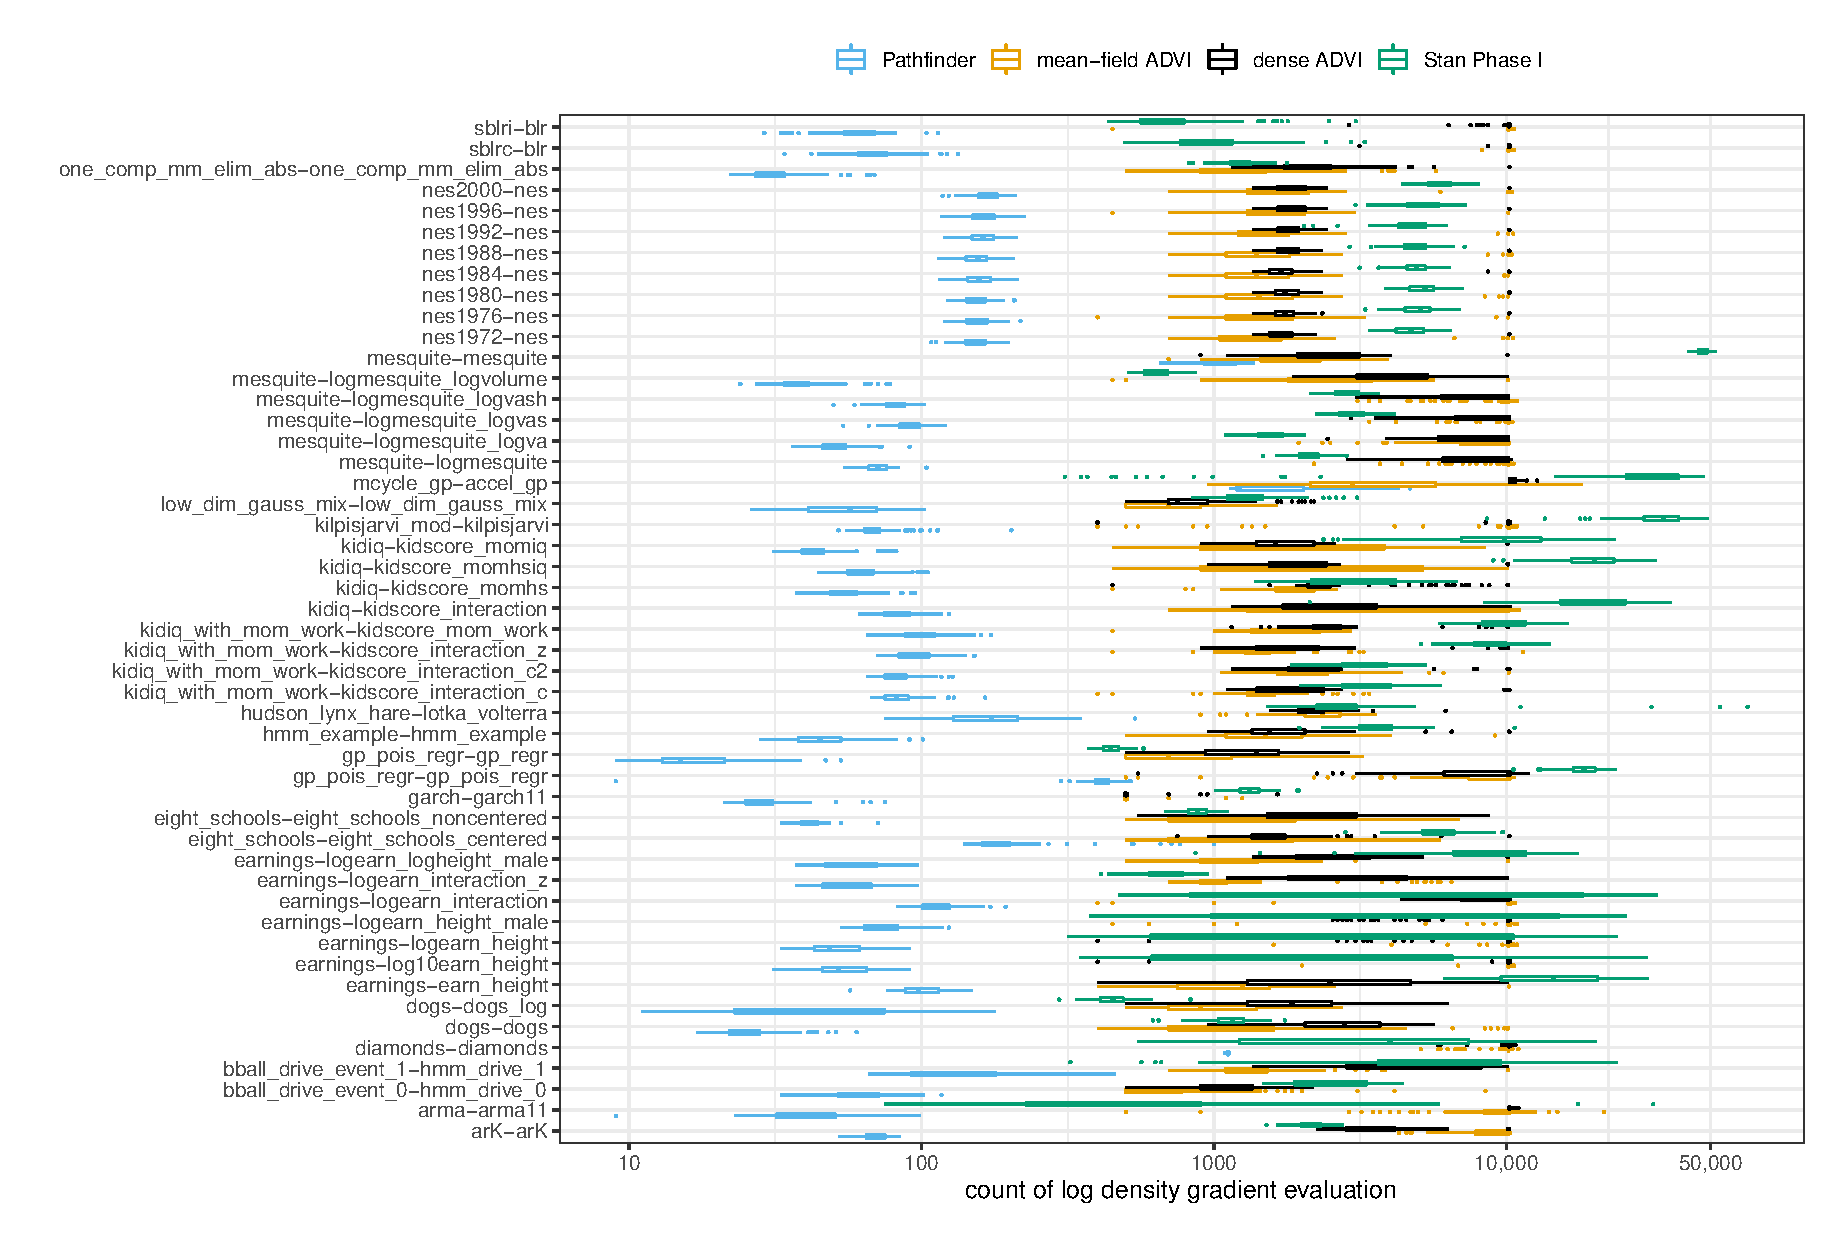
\includegraphics[width=0.6\textwidth]{img/log-density-evals.eps}
\end{center}
\vspace*{-10pt}
\begin{subitemize}
\item \myemph{1--3 orders of magnitude} fewer gradient (and log
  density) evaluations
\item \myemph{embarrassingly parallel} after L-BFGS (aside from a max operation) 
\end{subitemize}

\sld{But does it work?}
\begin{itemize}
\item sought a \myemph{neutral evaluation} not based on KL-divergence
  \begin{subitemize}
  \item KL-divergence is \myemph{asymmetric} (not a distance metric)
  \item KL-divergence as used favors \myemph{under-concentrated} approximations
  \end{subitemize}
\item we evaluate using \myemph{Wasserstein-1 distance} (aka ``earth mover's distance'')
  \begin{subitemize}
  \item proper \myemph{distance metric}
  \item \myemph{discrete optimal transport} problem solved in libraries
  \end{subitemize}
\item also \myemph{evaluate KL-divergence} (\textit{JMLR} editor Dave Blei told us reviewers would insist)
\end{itemize}

\sld{Wasserstein distance evaluation w.\ posteriordb}
\vspace*{-6pt}
\begin{center}
  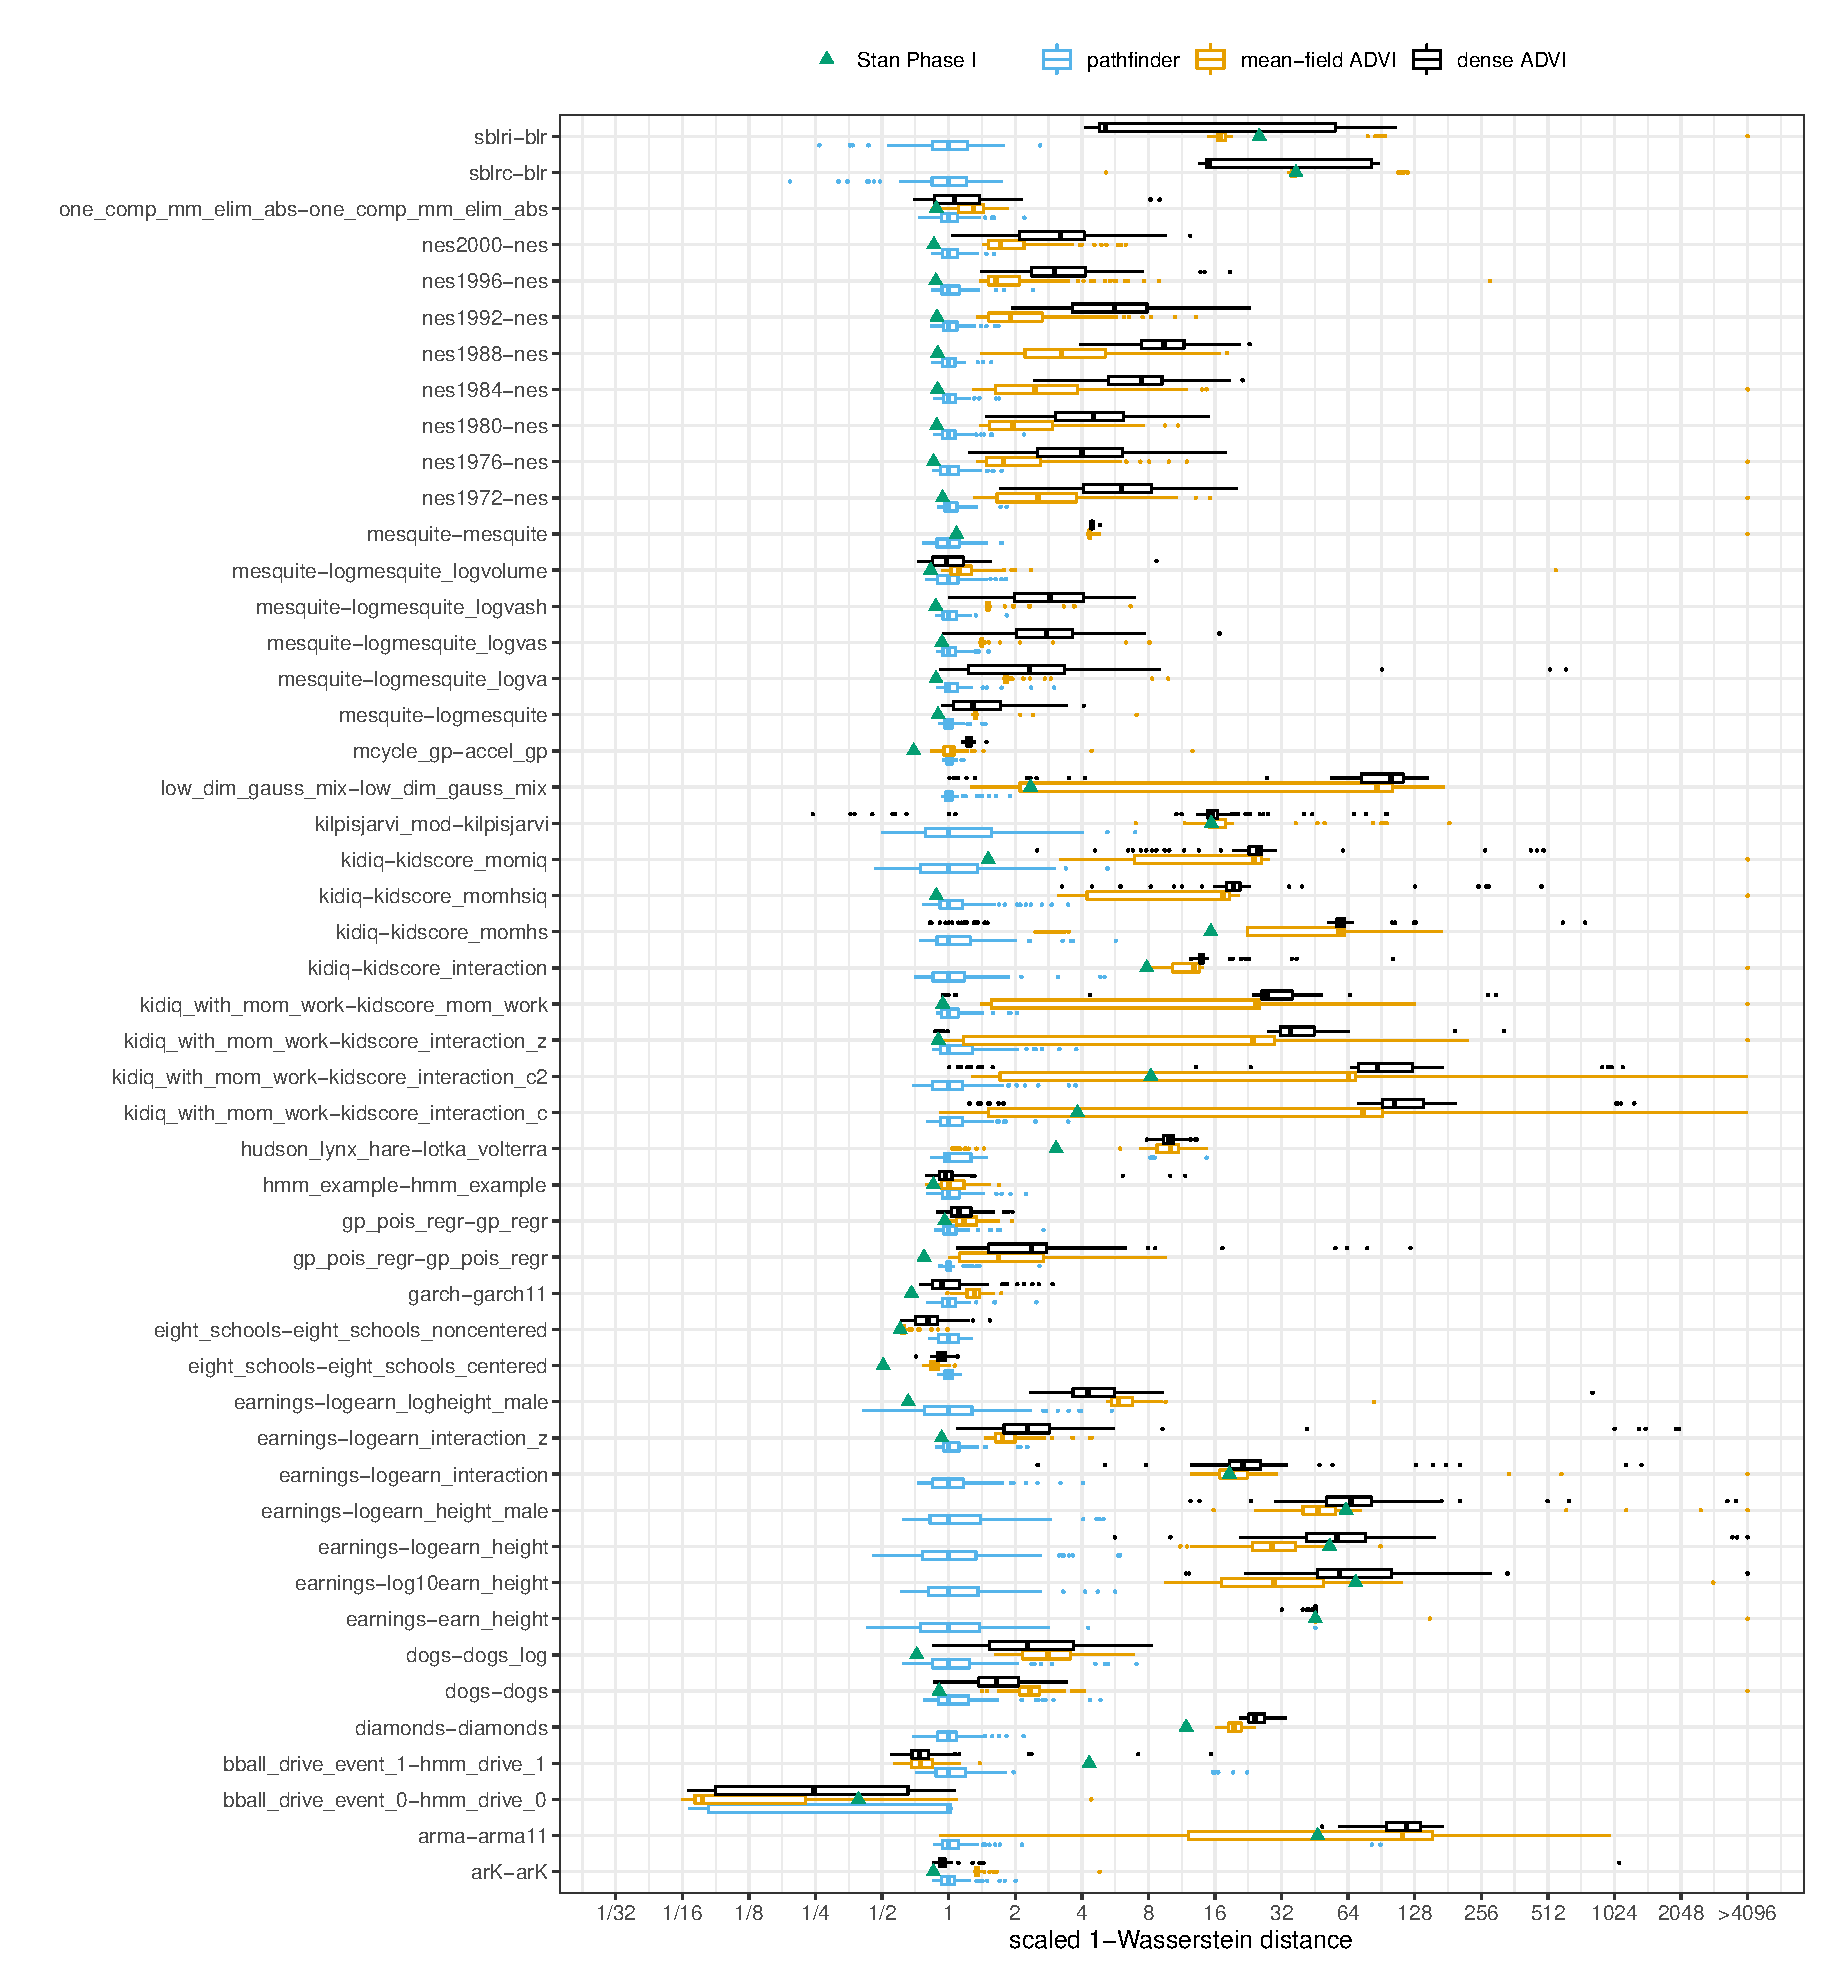
\includegraphics[width=0.4\textwidth]{img/wasserstein-eval.eps}
\end{center}
\vspace*{-6pt}
\begin{subitemize}
\item Pathfinder approximations are \myemph{better than ADVI} and \myemph{close to Stan Phase I}
\end{subitemize}


\sld{Is KL-divergence lower, too?}
\vspace*{-10pt}
\begin{center}
  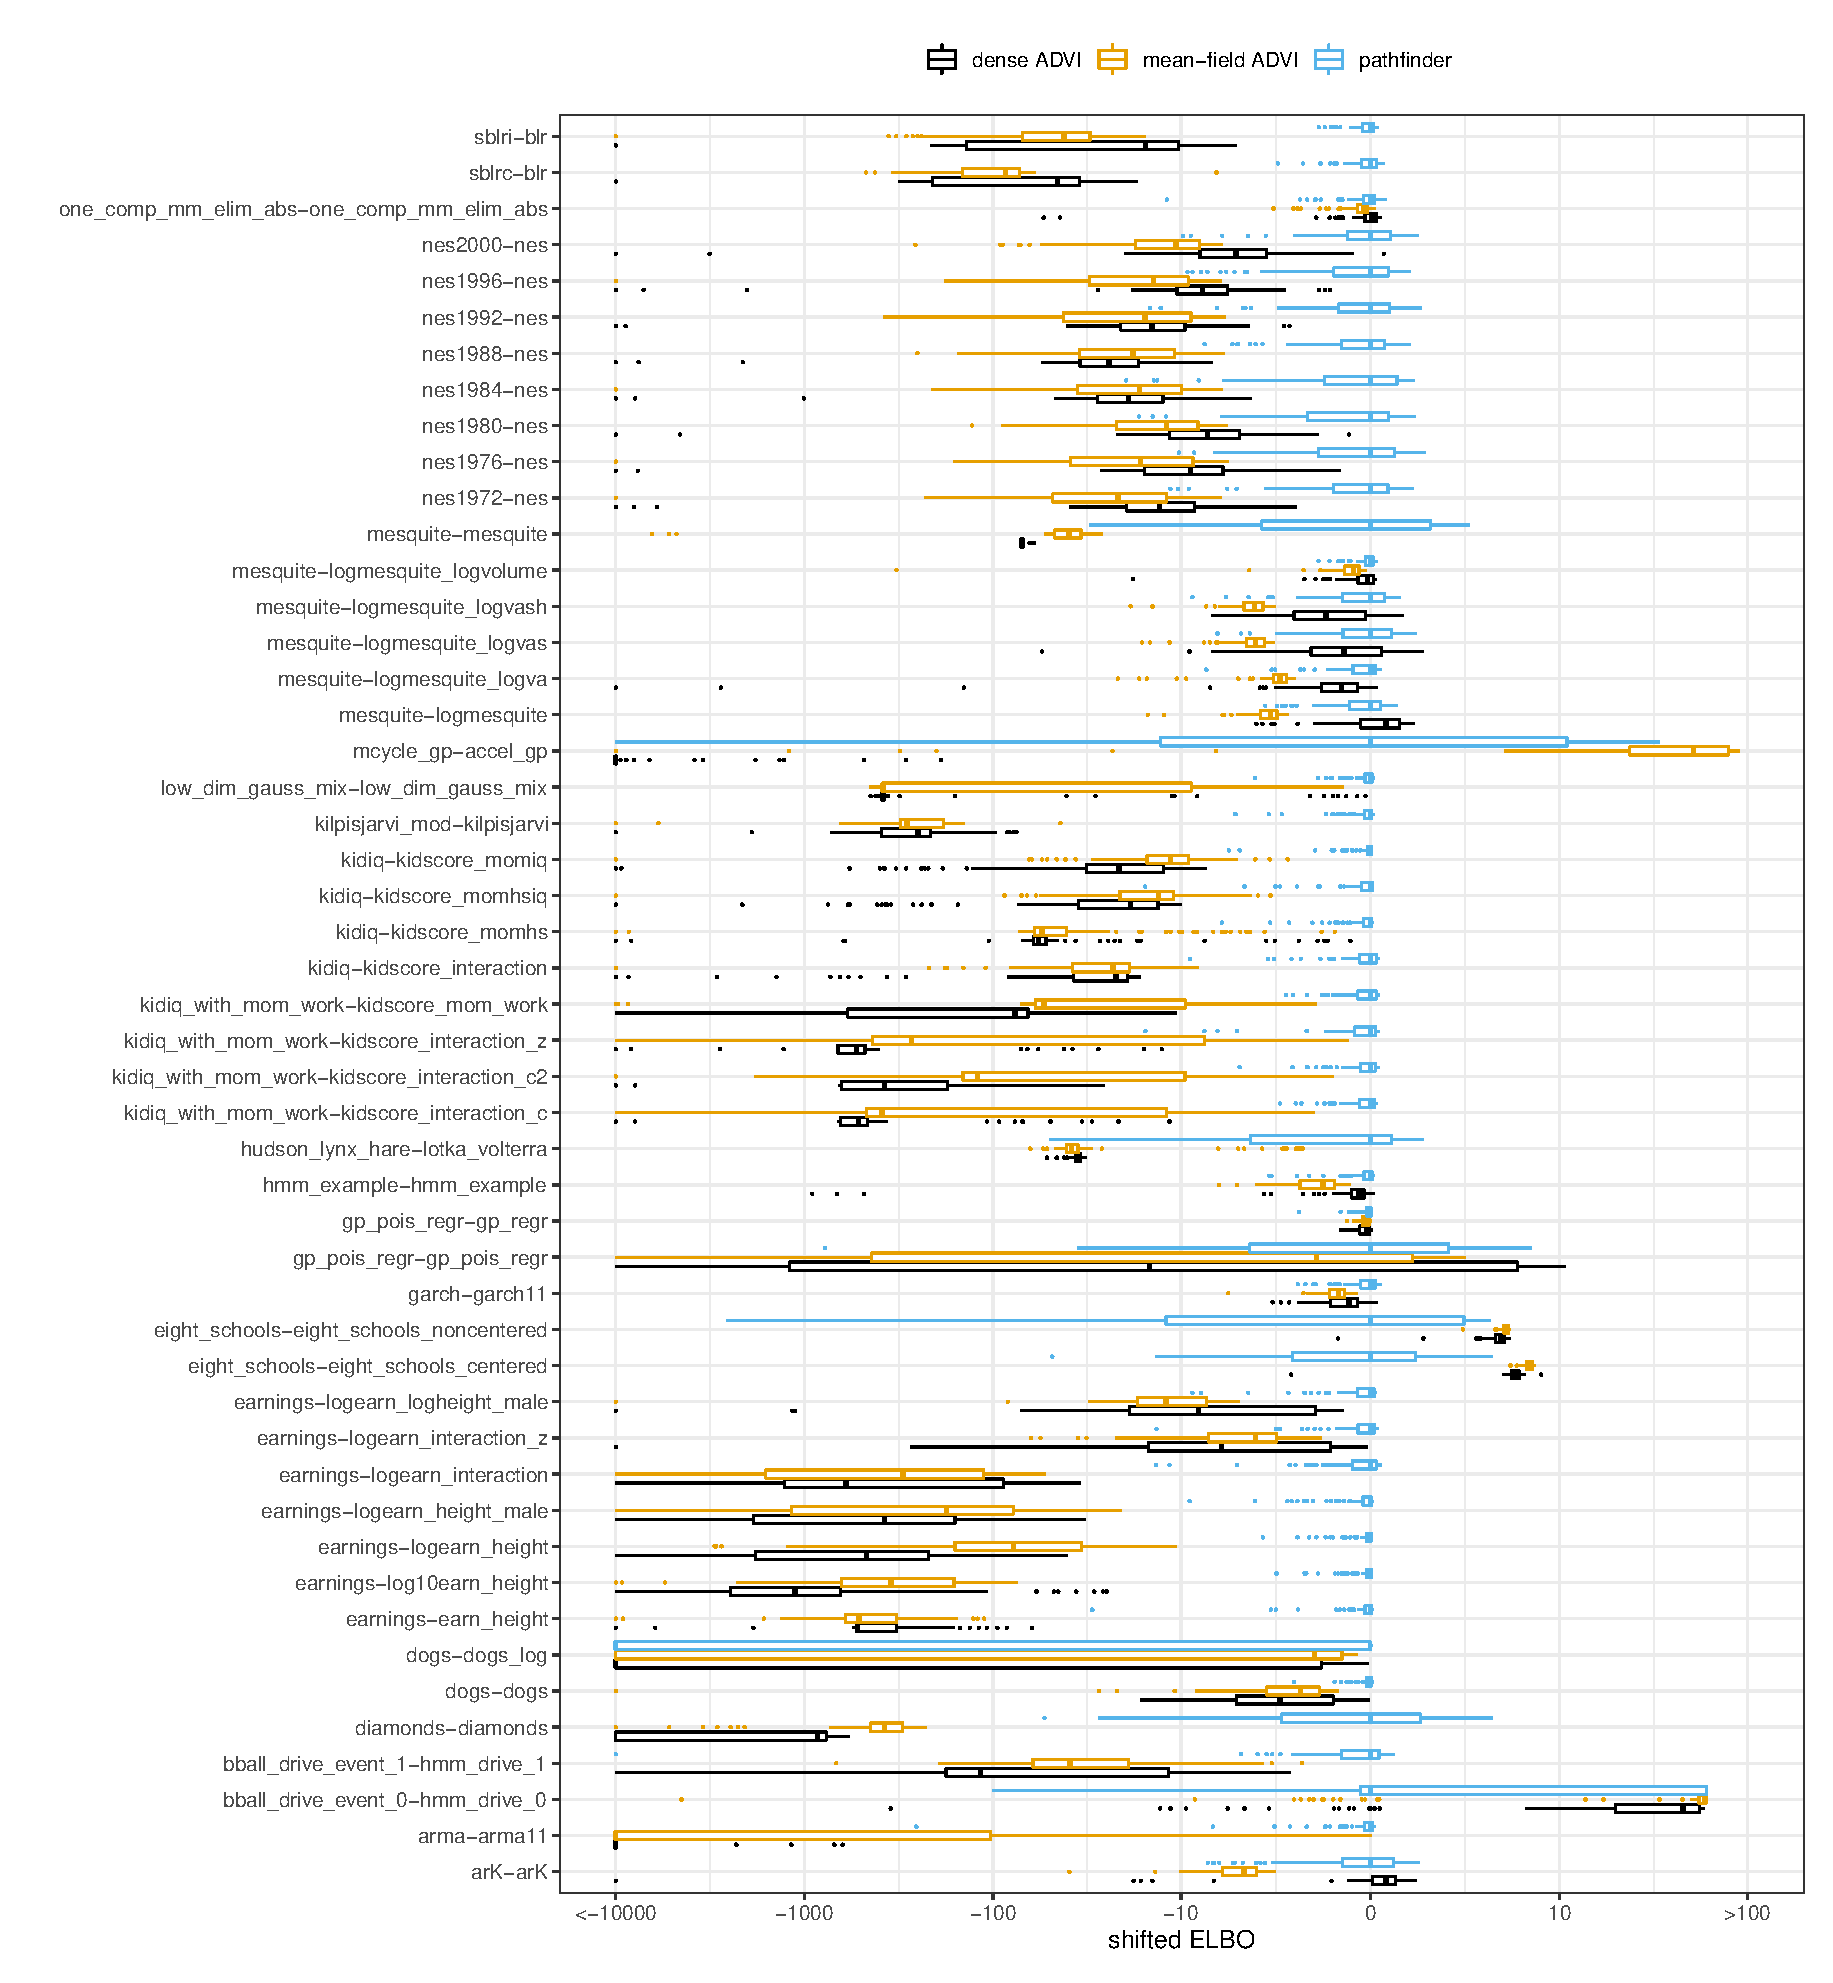
\includegraphics[width=0.4\textwidth]{img/elbo-eval.eps}
\end{center}
\vspace*{-10pt}
\begin{subitemize}
\item despite direct KL minimization,
  \myemph{ADVI optimization is unstable}
  \hfill (Vehtari et al.)
\item ELBO is negative KL-divergence plus constant (as shown earlier)
\end{subitemize}


\sld{Multi-path Pathfinder}
\begin{itemize}
\item sometimes L-BFGS gets \myemph{stuck in local optima} corresponding to a minor modes (i.e., low mass regions)
\item sometimes the posterior \myemph{isn't approximately normal} (e.g., low data, complex models)
\item \myemph{multi-path Pathfinder} runs multiple single-chain Pathfinder runs \myemph{in parallel}
\item \myemph{importance resamples} the draws (with \myemph{Pareto smoothing}) (very fast)
\item generalizes \myemph{variational family} to a \myemph{mixture of normals} (with low-rank plus diagonal covariance)
\end{itemize}

\sld{Importance sampling and resampling}
\begin{itemize}
\item \myemph{importance weight} for draw $\theta^{(m)}$ is
  \[
    w_m = \frac{p(\theta^{(m)} \mid y)}
    {q(\theta^{(m)} \mid \phi)}
  \]
\item \myemph{importance sampling} calculates estimates
  \[
    \mathbb{E}[f(\theta) \mid y]
    \approx \frac{1}{\textrm{sum}(w)} \sum_{m=1}^M w_m \cdot f(\theta^{(m)})
  \]
\item \myemph{importance resampling} draws a sample of size $M$
  \myemph{with replacement} from $\theta^{(1)}, \ldots, \theta^{(M)}$,
  with probabilities \myemph{proportional to weights}
\[
    p(\theta^{(m)}) \propto w_m
\]
\end{itemize}

\sld{Pareto smoothed importance (re)sampling}
\begin{itemize}
\item weights can have \myemph{high variance} (or even infinite) when proposal density $q$ is \myemph{far from target} density $p$
\item one approach is to \myemph{truncate} the weights, but \myemph{smoothing} is better
\item \myemph{fit Pareto} (power law) distribution to weights \hfill (Aki Vehtari et al.)
\item byproduct is a \myemph{goodness of fit} statistic $\widehat{K}$ \hfill (Yuling Yao et al.)
\item divide $(0, 1)$ into $M$ \myemph{evenly spaced} points
\item \myemph{map} points in $(0, 1)$ back to weights in $(0, \infty)$ with Pareto \myemph{inverse cdf}
\item \myemph{sort} the weights and \myemph{replace} with the Pareto-distributed points
\end{itemize}

\sld{Multi-path Pathfinder evaluation}
\vspace*{-10pt}
\begin{center}
  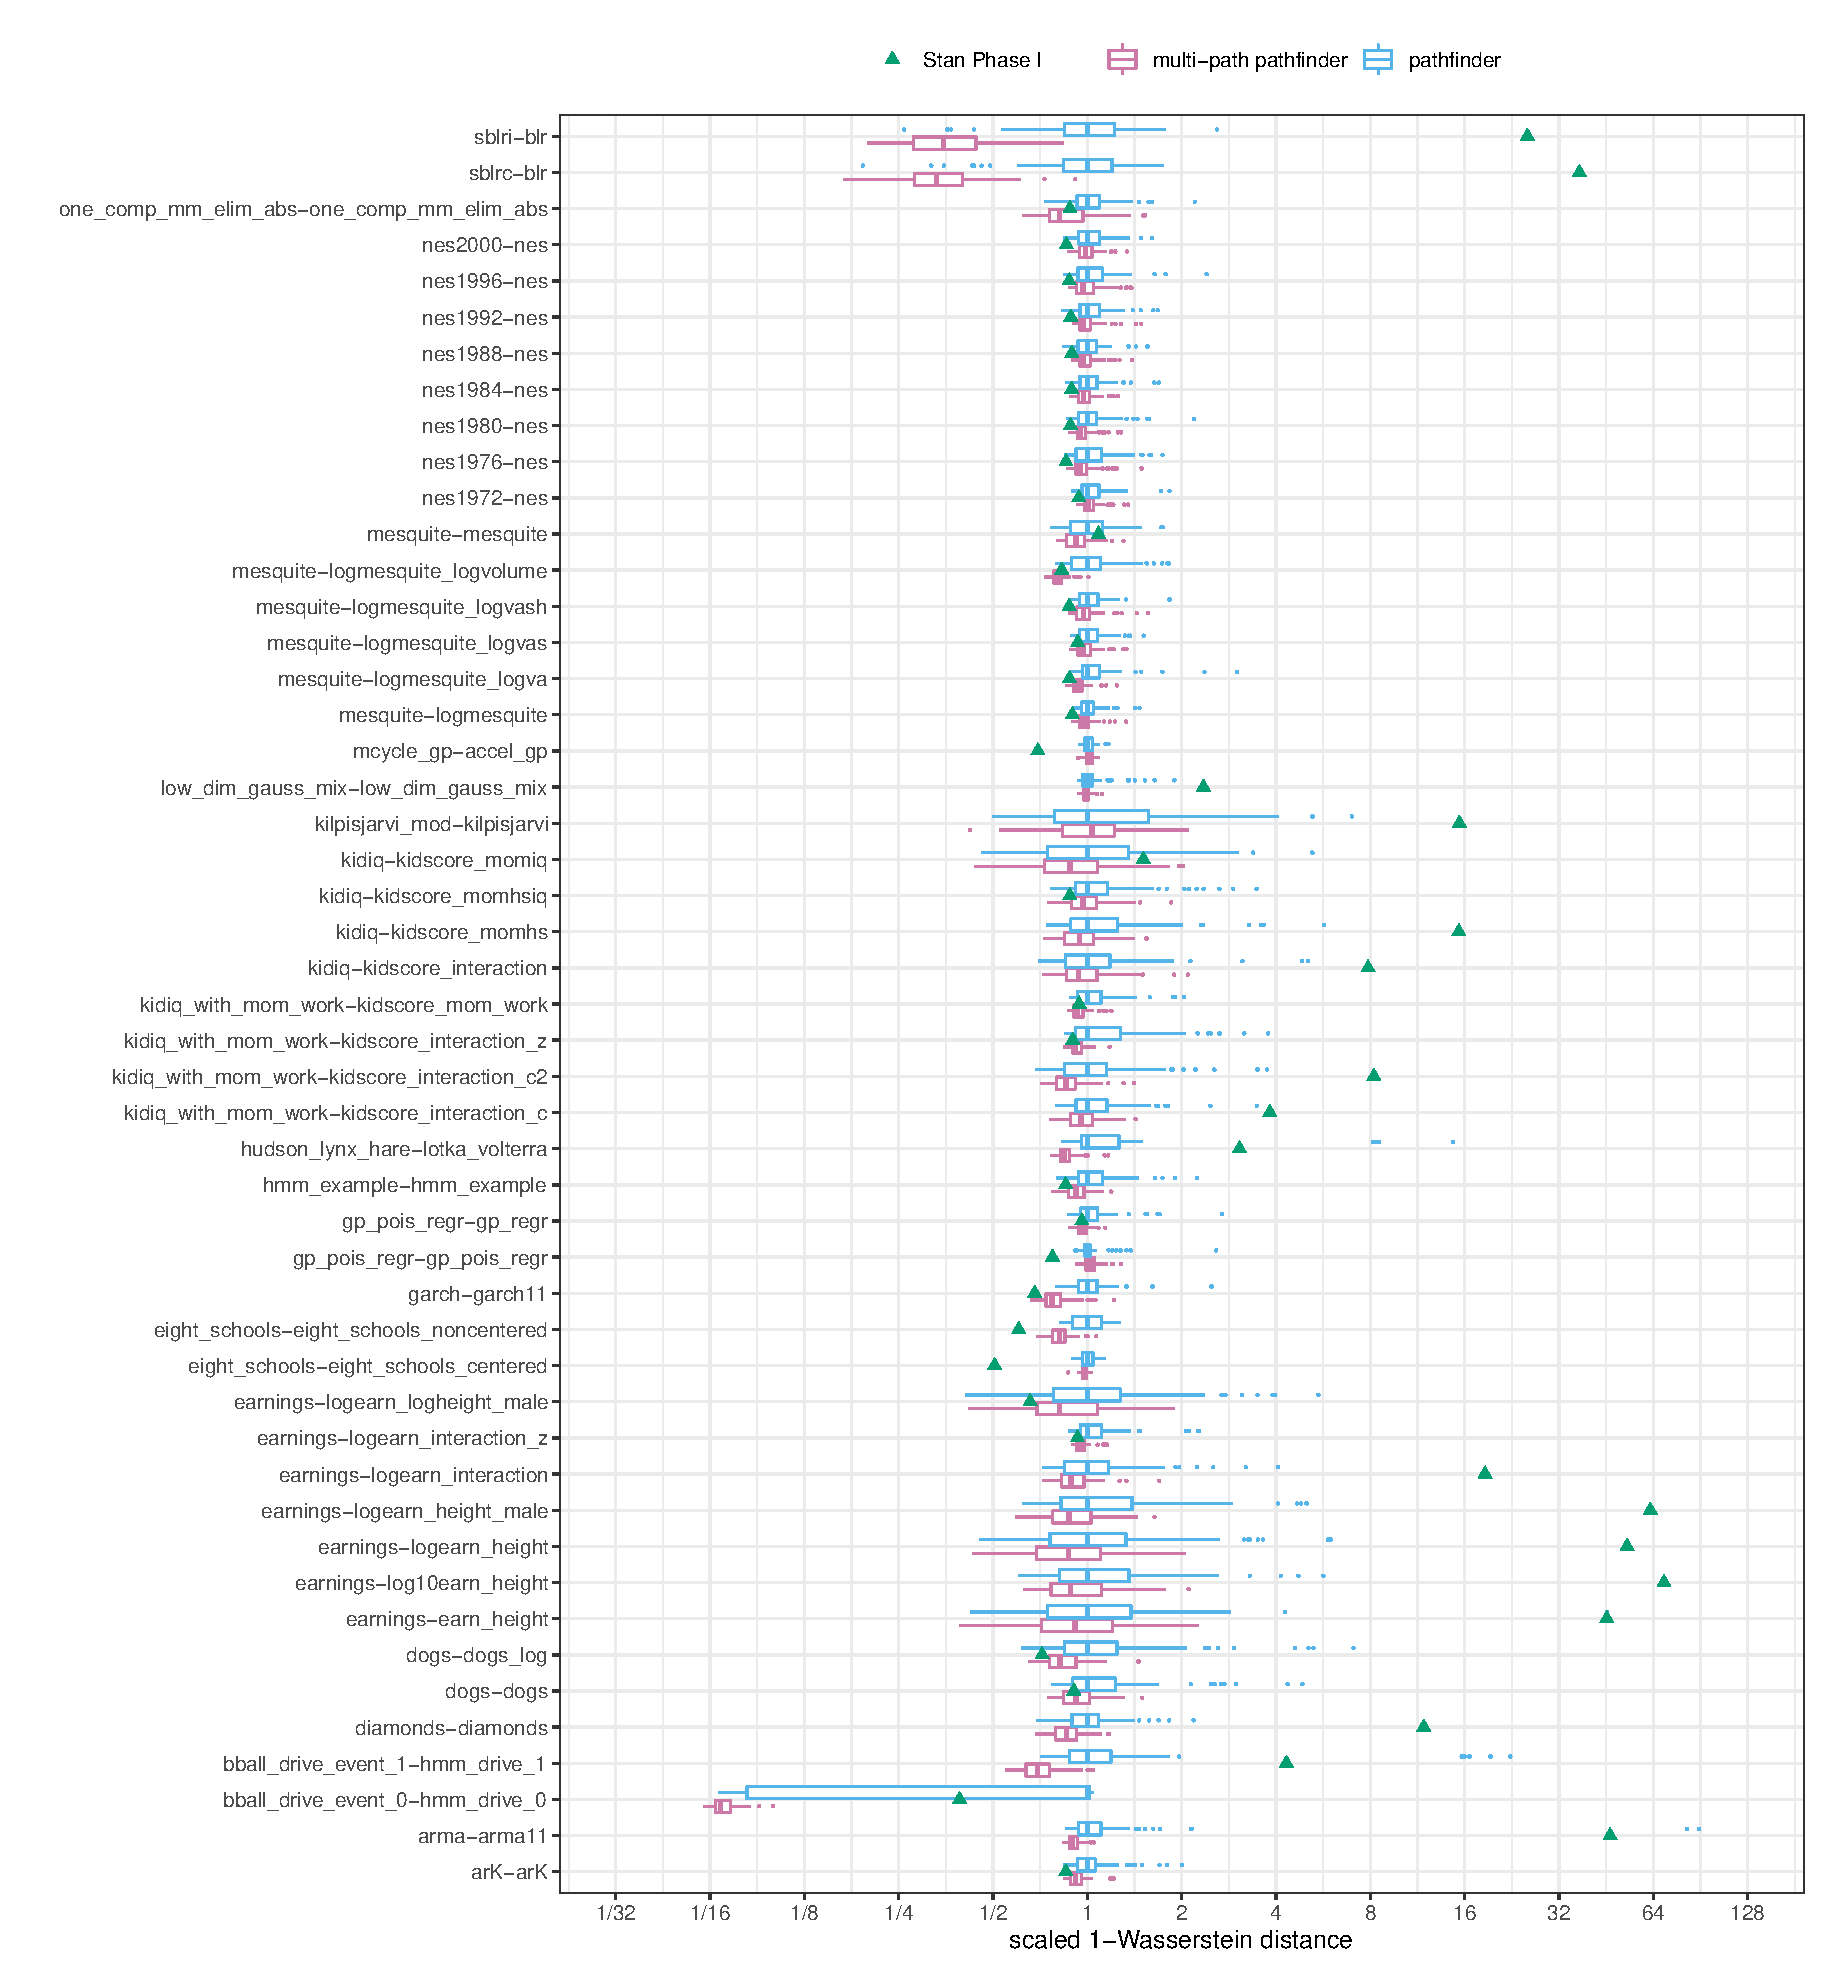
\includegraphics[width=0.45\textwidth]{img/multi-path-Wasserstein.eps}
\end{center}
\vspace*{-6pt}
\begin{subitemize}
\item multi-path is mostly \myemph{a bit better} but in some cases \myemph{much better}
\end{subitemize}



\end{document}


